%\chapter{Genome-scale metabolic network reconstruction of \textit{C. thermocellum} to design modular cells for consolidated bioprocessing} \label{ch:ctherm}
\chapter{Development of an updated genome-scale metabolic model of \textit{Clostridium thermocellum} and its application for integration of multi-omics datasets and modular cell design} \label{ch:ctherm}

\disclose{Development of an updated genome-scale metabolic model of Clostridium thermocellum and its application for integration of multi-omics datasets. Garcia, S., Thompson, R.A., Giannone, R. J., Dash, S., Maranas , C. D., and Trinh, C. T. In preparation, 2019}
Supplementary Material 1 is provided in Appendix \ref{apx:sm1-ctherm}, while Supplementary Files 2, 3, 4, and 5 are provided as attachments.


% Command to easily format gene knockouts
\makeatletter
\newcommand\ko[1]{{\@for\tmp:=#1\do{\textit{$\Delta$\tmp}}}}
%\newcommand\ko[1]{\textit{$\Delta$#1}}
\makeatother

% Math definitions
\newcommand\pFBA{\mathrm{pFBA}}
\newcommand\FVA{\mathrm{FVA}}
\renewcommand\sim{\mathrm{sim}}
\newcommand\meas{\mathrm{meas}}
\newcommand\FC{\mathit{FC}}

\section*{Abstract}
    Solving environmental and social challenges such as climate change requires a shift from our current non-renewable manufacturing model to a sustainable bioeconomy.
    A promising technology to enable carbon neutral production of energy and materials from plant biomass is consolidated bioprocessing (CBP). The most promising CBP organism identified thus far is \textit{Clostridium thermocellum}, a thermophilic microbe capable of efficient degradation of untreated lignocellulosic biomass to produce biofuels and biomaterials.
    However, the complex metabolism of \textit{C.~thermocellum} is not fully understood, hindering metabolic engineering to achieve high rates, titers, and yields of valuable molecules.
    In this study, we developed an updated genome-scale model of \textit{C.~thermocellum} that accounts for recent metabolic findings, has improved prediction accuracy, and is standard-conformant to ensure easy reproducibility.
    We illustrated two of the many uses of the developed genome-scale model: First, we applied the model to study biotechnologically relevant mutants for ethanol production. This analysis was done with a novel quantitative multi-omics integration protocol that led to interesting findings in redox stress metabolism, providing new engineering targets for the production of reduced molecules. Second, we used the model to design modular platform strains for efficient production of alcohols and esters. The proposed designs not only feature intuitive push and pull metabolic engineering strategies, but also novel manipulations around important central metabolic branch-points.
    We anticipate the new model will become a useful tool for metabolic engineering and systems biology of \textit{C.~thermocellum}.

%\section*{Highlights}
%\begin{itemize}
%    \item Developed iCBI655, a genome-scale model that coherently reflects the most current genetic and metabolic knowledge of the consolidated bioprocessing organism \textit{Clostridium thermocellum}.
%    \item Trained the iCBI655 model against  a comprehensive dataset of extracellular fluxes and known lethal genotypes and conditions, leading to enhanced prediction accuracy of growth phenotypes across culture conditions.
%    \item The iCBI655 model emphasizes accessibility and reproducibility through standard-conformance, interactive metabolic maps, and comprehensive documentation.
%    \item Multi-omics integration method was developed and applied it to proteomics and extracellular flux datasets for ethanol over-producing hydrogenase deletion mutants, revealing the importance of NADPH biosynthesis in response to redox stress.
%\end{itemize}

\section{Introduction}
Global oil reserves will be depleted soon,\citep{shafiee2009}
and climate change could become a major driver of civil conflict.\citep{hsiang2011}
These challenges to security and the environment need to be addressed by replacing our current non-renewable production of energy and materials for a renewable and carbon neutral approach.\citep{ragauskas2006}
The thermophilic bacterium \textit{C.~thermocellum} is capable of efficient degradation of lignocellulosic biomass to produce biofuels and biomaterial precursors, making this organism an exceptional candidate for biocatalysis.\citep{olson2012}
However, its complex and poorly understood metabolism remains the main roadblock to achieve industrially competitive yields and titers of useful metabolites, including biofuels such as ethanol\citep{tian2016} and isobutanol.\citep{lin2015}
To support metabolic engineering efforts of \textit{C.~thermocellum} in the last decade, several genome-scale models (GSMs) of metabolism have been developed.

The first GSM of \textit{C.~thermocellum}, named iSR432, was developed for strain ATCC27405  and applied to identify gene deletion strategies for high ethanol yield. \citep{roberts2010}
More recently, Thompson et al.\ developed the iAT601 genome-scale model \citep{thompson2016} for strain DSM1313, the current engineering platform strain due to better availability of genetic engineering tools.\citep{argyros2011}
The iAT601 model was used to identify genetic manipulations for high ethanol, isobutanol, and hydrogen production,\citep{thompson2016} and to understand growth cessation prior to full substrate depletion observed under high-substrate loading fermentations that simulate industrial conditions.\citep{thompson2017}
In addition to these core and genome-scale steady-state metabolic models, a kinetic model of central metabolism, k-ctherm118, was recently developed and used to elucidate the mechanisms of nitrogen limitation and ethanol stress.\citep{dash2017} Due to the biotechnological relevance of the Clostridium genus, GSMs have also been developed for other species,\citep{dash2016} including
\textit{C. acetubutylicum},\citep{lee2018, senger2008, salimi2010, mcanulty2012, wallenius2013, dash2014, yoo2015}
\textit{C. beijerinckii},\citep{milne2011}
\textit{C. butyricum},\citep{serrano2017}
\textit{C. cellulolyticum},\citep{salimi2010}
and \textit{C.ljungdahlii}.\citep{nagarajan2013}


In this study, we developed an updated genome-scale model of \textit{C.~thermocellum}, named iCBI655, with more comprehensive and precise metabolic coverage, enhanced prediction accuracy, and extensive documentation. This model is a human curated database that coherently represents all the available genetic, genomic, and metabolic knowledge of \textit{C.~thermocellum} from both experimental literature and bioinformatic predictions. Consequently, the model not only enables metabolic flux simulation but also provides a framework to contextualize disparate datasets at the system level. To this end, we developed a quantitative multi-omics integration method and applied it to well-known biotechnological mutants for ethanol production, leading to new insights in redox stress mechanisms and potential engineering targets for enhanced production of reduced molecules. Furthermore, we also used the model,
in combination with the previously proposed ModCell tool, \citep{garcia2019,garcia2020b}
to design modular platform strains\citep{garcia2019b} for alcohol and ester production.

\section{Results}
\subsection{Development of an upgraded \textit{C.~thermocellum} genome-scale model named iCBI655}
The iCBI655 model was developed using the published iAT601 model\citep{thompson2016} as a starting point. The enhancements with respect to the previous model include updated metabolic pathways, new annotation, and new extensive documentation.
A detailed account of these changes can be found in the Supplementary Material~\ref{sm:code}. Here, we highlight the most relevant modifications.

\subsubsection{Modeling updates}
To facilitate model usage and reduce the chances of human error, the identifiers of reactions and metabolites were converted from KEGG into BiGG human-readable form.\citep{king2015}
Additionally, reaction and metabolite identifiers were also linked to the modelSEED database \citep{henry2010} that enables analysis through the KBase web interface. \citep{arkin2018}
The gene identifiers and functional descriptions were updated to the most current annotation (NCBI Reference Sequence: NC\_017304.1). %(identifiers changed from Clo1313\_xxx to CLO1313\_RSxxx).
Metabolite formulas and charges from the modelSEED database\citep{henry2010} were included in the model and reactions were systematically corrected for charge and mass balance by the addition of protons and water.


\subsubsection{Metabolic updates}

The automated construction process used in the previous model introduced several inconsistencies that were corrected in the current model. We removed reactions that were blocked and non-gene-associated, apparently introduced during automated gap-filling. Two notable examples are i) the blocked selenate pathway which lacks experimental evidence (e.g., selenoproteins have not been found in \textit{C.~thermocellum}), and ii) blocked reactions involving molecular oxygen (e.g., oxidation of Fe$^{2+}$ to Fe$^{3+}$) that are not possible in strict anaerobes. Furthermore, tRNA cycling reactions were unblocked by including tRNA into the biomass reactions.\citep{reimers2017}
Metabolite isomers were examined and consolidated under the same metabolite identifier when possible, leading to the removal of duplicated reactions and the elimination of gaps.
Transport and exchange reactions were updated to reflect the export of amino acids and uptake of pyruvate as observed during fermentation experiments.\citep{holwerda2014}

In terms of specific reactions, oxaloaceate decarboxylase was eliminated from the model in accordance with recent findings.\citep{olson2017}
The stoichiometries of pentose-phospate reactions sedoheptulose 1,7-bisphosphate D-glyceraldehyde-3-phosphate-lyase (FBA3) and sedoheptulose 1,7-bisphosphate ppi-dependent phosphofructokinase (PFK3\_ppi) were corrected (according to experimental evidence\citep{rydzak2012}) from the previous model by ensuring mass balance and avoiding lumping multiple steps into one reaction.
Transaldolase (TALA) was removed from the model due to lack of annotation for this gene in \textit{C.~thermocellum} and to also ensure PFK essentiality as observed experimentally (personal communication from Lynd Research Lab, Dartmouth College).

% Bioenergtics/hydrogenases
Several modifications were also performed in key bioenergetic reactions.
The reactions catalyzed by membrane-bound enzymes inorganic diphosphatase (PPA) \citep{zhou2013} and
membrane-bound ferredoxin-dependent hydrogenase (ECH)\citep{calusinska2010}
were corrected to capture proton translocation.
Furthermore, hydrogenase reactions were updated to ensure ferredoxin association for all cases and remove those reactions which do not involve ferredoxin and only use NAD(P)H as cofactor based on our recent understanding of \textit{C.~thermocellum} metabolism.\citep{biswas2017} % TODO: This is one of Satya's changes but the reference seems odd to me, maybe asking him when sending out the manuscript.
Gene-protein-reaction associations logical relationships were updated to
represent experimental knowledge, e.g., the hydrogenases BIF (CLO11313\_RS09060-09070) and H2ASE (CLO1313\_RS12830, CLO1313\_RS02840) require of the maturase Hyd (CLO1313\_RS07925, CLO1313\_RS11095, CLO1313\_RS12830) to be functional, and the maturase itself requires all of its subunits to operate. This enables accurate representations of \textit{hydG} deletion genotypes.\citep{biswas2015}

%Hypothetical
Two hypothetical reaction modifications were introduced to ensure consistency with reported phenotypes:
i) To enable growth without the need for succinate secretion, as observed in experimental data (Supplementary Material \ref{sm:datasets}), the reaction homoserine-O-trans-acetylase (HSERTA) was added to enable methionine biosynthesis (essential for growth) without succinate formation.
Although this reaction is not currently known to be associated with any gene in \textit{C.~thermocellum}, it is known to be present in other clostridial GSMs. \citep{nagarajan2013}
ii) The reaction deoxyribose-phosphate aldolase (DRPA) was removed to ensure correct lethality prediction of the \ko{hydG,ech,pfl} as well as the correct prediction of growth recovery in this mutant by addition of external electron sinks such as sulfate or ketoisovalerate (Table~\ref{tab6:mutants}). DRPA  was identified as the best target for removal from a systematic single-reaction deletion analysis (Section \ref{sec:deletion_analysis}).
Deletion of \textit{hydG}, \textit{ech}, and \textit{pfl}  are proven strategies for enhanced product synthesis while preserving cellular growth, \citep{biswas2015, thompson2015, tian2016}
thus the correct prediction of \ko{hydG,ech,pfl}-associated phenotypes is critical to successfully use the model for computational strain design.\citep{long2015, ng2015, maranas2016, wang2018,garcia2019, garcia2019b, garcia2019c}

\begin{table}[ph]
    \caption[Comparison of mutant growth rate prediction between iAT601 and iCBI655 models]{Comparison of mutant growth rate prediction between iAT601 and iCBI655. To simulate mutant genotypes for growth rate prediction, gene deletions were applied and growth rate was maximized without constraining secretion fluxes to known values, to recreate simulations for strain design were such additional constraints are not available. \textit{In vivo} values are taken form Thompson et al.\citep{thompson2015}, where in some mutants growth rate was not reported, but growth recovery was reported, this is indicated with the ``+" symbol.}
    \centering
    \rowcolors{2}{gray!25}{white}
\resizebox{\textwidth}{!}{\begin{tabular}{>{\em}lllllc}
\toprule
\normalfont{Gene deletions}	& Medium 	& \multicolumn{3}{l}{Fraction of W.T. growth rate (\%)} 	\\
		&			& \textit{iAT601}	& \textit{iCBI655}	& \textit{In vivo}  	\\
\midrule
hydg         	& MTC                  	& 100      	& 100 		& 73	\\
hydg-ech     	& MTC                   & 85       	& 85 		& 67 	\\
hydg-pta-ack 	& MTC           	& 100       	& 100		& 48 	\\
hydG-ech-pfl	& MTC			& 58       	& 0		& 0	\\
hydG-ech-pfl	& MTC + fumarate	& 377		& 726 		& 0	\\
hydG-ech-pfl	& MTC + sulfate		& 58       	& 65		& +	\\
hydG-ech-pfl	& MTC + ketoisovalerate & 97       	& 101		& +	\\
\hline
\end{tabular}}

% In the fumarate addition case the over-prediction if growth is due to FUM, Fumarase, (mal__L <=> fum + h2o), if this reaction is removed, then growth prediction is 100%. Alternatively the fumarate uptake rate might be limited. Fumarase also operates close to equilibrium (see equilibrator), so that might be another rate limiting factor.

% Annotation
% + indicates the mutants grow

% Notes:
% - For in vivo calculations, the average growth rate value was used.
% - all mediums use cellobiose

% Calculation of growth rate for Tian2016
% - Quote from Tian2016: "To examine strain improvements via evolution, the wild type and resulting three strains (AG553, AG601, and LL1210) were cultivated in serum bottles in defined medium. Maximum growth rate was determined on 5 g/L cellobiose (Table 1). The wild-type strain had the fastest growth rate, while the growth rate of the unevolved strain AG553 was the slowest." However the wild-type growth rate is not reported. A reference to Papaneck 2015 is provided.
% - quote from Papaneck 2015 (which Tian2016 cites as the source of its strains): "While wild type C. thermocellum grew at a rate of 0.14±0.03 h−1, strain AG553 experienced a substantially longer lag phase and had an initial growth rate of 0.03±0.01 h−1. After reaching approximately an OD of 0.15, the growth rate increased to 0.13±0.02 h−1" This paper uses MTC
% - Tian reports average growth rates for the mutant of 0.06 before adaptation, 0.10 after one round of adpatation, and 0.22 after a second round of adaptation.  While the adaptation procedures differ, all growth rates are characterized under the same MTC medium with 5 g/L of cellobiose. The initial and final growth rates are reported.

% References
%[1] Thompson, R. Adam, et al. "Elucidating central metabolic redox obstacles hindering ethanol production in Clostridium thermocellum." Metabolic engineering 32 (2015): 207-219.
%[2] Tian, Liang, et al. "Simultaneous achievement of high ethanol yield and titer in Clostridium thermocellum." Biotechnology for biofuels 9.1 (2016): 116.
%[3] Van Der Veen, Douwe, et al. "Characterization of Clostridium thermocellum strains with disrupted fermentation end-product pathways." Journal of industrial microbiology & biotechnology 40.7 (2013): 725-734.
%[related to 2] Papanek, Beth, et al. "Elimination of metabolic pathways to all traditional fermentation products increases ethanol yields in Clostridium thermocellum." Metabolic engineering 32 (2015): 49-54.

% Notes about additional growth rate data:
% Ref 1 data can be extracted from figure/ Raw data
% Ref 3 data can be extracted from figure 1




% Earlier versions:

% v1
%\rowcolors{2}{gray!25}{white}
%\resizebox{\textwidth}{!}{\begin{tabular}{>{\em}llllll}
%\toprule
%\normalfont{Gene deletions}	& Medium 	& \multicolumn{3}{l}{Fraction of W.T. growth rate}	& Reference \\
%		&			& iAT601	& iCBI655	& \textit{In vivo} & 		\\
%\midrule
%hydg         	& MTC                  	& 100.0\%       & 100.0\% 	& 72.7\%	& \cite{thompson2015} \\
%hydg-ech     	& MTC                   & 85.0\%        & 84.0\% 	& 66.6\% 	& \cite{thompson2015} \\
%hydg-pta-ack 	& MTC           	& 100.0\%       & 100.0\%	& 48.5\% 	& \cite{thompson2015} \\
%hydG-ech-pfl	& MTC			& 58.3\%	& 0\%		& 0\%		& \cite{thompson2015} \\
%hydG-ech-pfl	& MTC + fumarate	& 376.6\%	& 101.7\%	& 0\%		& \cite{thompson2015} \\
%hydG-ech-pfl	& MTC + sulfate		& 58.3\%	& 64.3\%	& +		& \cite{thompson2015} \\
%hydG-ech-pfl	& MTC + ketoisovalerate & 96.6\%	& 101.1\%	& +		& \cite{thompson2015} \\
%hydG-pfl-ldh-pta-ack &	MTC		& 94.1\%	& 77.7\%	& 42.85\%/157.1\%	& \cite{tian2016} \\
%ldh		& MTC			& 100.0\%	& 100.0\%	& \textasciitilde100\%	& \cite{van2013} \\
%pta-ack		& MTC			& 100.0\%	& 100.0\%	& +		& \cite{van2013} \\
%ldh-pta-ack	& MTC			& 100.0\%	& 100.0\%	& +/+		& \cite{van2013} \\
%\hline
%\end{tabular}}

%v2
%\rowcolors{2}{gray!25}{white}
%\resizebox{\textwidth}{!}{\begin{tabular}{>{\em}lllllc}
%\toprule
%	\normalfont{Gene deletions}	& Medium 	& \multicolumn{3}{l}{Fraction of W.T. growth rate (\%)}	& Reference \\
%		&			& iAT601	& iCBI655	& \textit{In vivo} & 		\\
%\midrule
%hydg         	& MTC                  	& 100      	& 100 		& 73	& \cite{thompson2015} \\
%hydg-ech     	& MTC                   & 85       	& 84 		& 67 	& \cite{thompson2015} \\
%hydg-pta-ack 	& MTC           	& 100       	& 100		& 48 	& \cite{thompson2015} \\
%hydG-ech-pfl	& MTC			& 58       	& 0		& 0		& \cite{thompson2015} \\
%hydG-ech-pfl	& MTC + fumarate	& 377		& 102		& 0		& \cite{thompson2015} \\
%hydG-ech-pfl	& MTC + sulfate		& 58       	& 64		& +		& \cite{thompson2015} \\
%hydG-ech-pfl	& MTC + ketoisovalerate & 97       	& 101		& +		& \cite{thompson2015} \\
%hydG-pfl-ldh-pta-ack &	MTC		& 94       	& 78		& 43/157	& \cite{tian2016} \\
%ldh		& MTC			& 100		& 100		& \textasciitilde100	& \cite{van2013} \\
%pta-ack		& MTC			& 100		& 100		& +		& \cite{van2013} \\
%ldh-pta-ack	& MTC			& 100		& 100		& +/+		& \cite{van2013} \\
%\hline
%\end{tabular}}

    \label{tab6:mutants}
\end{table}



% Probably not worth noting:
%%%%%%%%%%%%%%%%%%%%%%%%%%%
% - based on genome annotation, a sodium-translocating PPA was added.
% - reactions featuring generic metabolites were deleted.

\subsection{Comparison of iCBI655 against other genome-scale models}
We compared iCBI655 with the previous GSMs of \textit{C.~thermocellum} and the highly-curated GSM iML1515 of the extensively studied bacterium \textit{Escherichia coli} (Table~\ref{tab6:models}).
The increased number of genes in iCBI655 with respect to iAT601 cover a variety of functions, including hydrogenase chaperons, cellulosome and cellulase, ATP synthase, and transporters.
Remarkably, iCBI655 has a smaller percentage of blocked reactions than iAT601, indicating higher biochemical consistency. The number of metabolites in iCBI655 was smaller than those in iAT601 due mainly to the removal of metabolites that did not appear in any reaction, duplicated metabolites (e.g., certain isomers), and blocked pathways added automatically during gap-filling but that lack any gene association. \textit{C.~thermocellum} DSM1313 has 2911 protein coding genes, although not all are metabolic, of which iCBI655 covers 22\%, while \textit{E.~coli} MG1655 has 4240 genes of which iML1515 covers 35\%. Overall, iCBI655 increases the coverage of the metabolic functionality of \textit{C.~thermocellum} but remains far from the highly studied \textit{E.~coli}.


\begin{table}[h]
    \caption[Comparison of all genome-scale models of \textit{C.~thermocellum}]{Comparison of all genome-scale models of \textit{C.~thermocellum} and the latest \textit{E.~coli} genome-scale model.}
    \centering
    \rowcolors{2}{gray!25}{white}
\resizebox{\textwidth}{!}{\begin{tabular}{llllll}
\toprule
		& iSR432 	& iCth446	& iAT601 	& iCBI665 & iML1515 \\
\midrule
Strain 		& ATCC27405 	& ATCC27405 	& DSM1313 	& DSM1313 & MG1655 \\
Genes		& 432 		& 446 		& 601 		& 665 	& 1515 \\
Metabolites 	& 583 		& 599 		& 903 		& 795 	& 1877 \\
Reactions 	& 632 		& 660 		& 872 		& 854 	& 2712\\
Blocked reactions & 39.2\% 	& 32.1\% 	& 40.8\% 	& 35.1\% & 9.8\% \\
%Lethal reactions & 20.1\%	& 20.0\% 	& 17.1\%	& 16.5\% & 4.46\% \\
	Reference 	& \cite{roberts2010} 	& \cite{dash2017} 	& \cite{thompson2016} & This study & \cite{monk2017}\\
\hline
\end{tabular}}

% For lethal reactions growth rate is reduced below 0.01. It should rather be defined as a % of the w.t. predicted growth.

% References:
%[1]	Roberts, Seth B., et al. "Genome-scale metabolic analysis of Clostridium thermocellum for bioethanol production." BMC systems biology 4.1 (2010): 31.
%[2]	Dash, Satyakam, et al. "Development of a core Clostridium thermocellum kinetic metabolic model consistent with multiple genetic perturbations." Biotechnology for biofuels 10.1 (2017): 108.
%[3]	Thompson, R. Adam, et al. "Exploring complex cellular phenotypes and model-guided strain design with a novel genome-scale metabolic model of Clostridium thermocellum DSM 1313 implementing an adjustable cellulosome." Biotechnology for biofuels 9.1 (2016): 194.
%[4]	Monk, Jonathan M., et al. "iML1515, a knowledgebase that computes Escherichia coli traits." Nature biotechnology 35.10 (2017): 904.
%

    \label{tab6:models}
\end{table}


\subsection{Training of model parameters under diverse conditions}
% Important point to make is that we intend to find a general, rather than specific value for gam/ngam
% Another thing to make clear is that these values while they intend to represent an actual biochemical event should be seen as model parameters.

Growth and non-growth associated maintenance (GAM and NGAM) are parameters that capture the consumption of ATP towards cell division and survival, respectively. These are known to be condition-specific, however, genome-scale models do not include a mechanistic description that allows to determine these ATP consumption rates as part of the simulation. Instead, GAM is incorporated into the biomass pseudo-reaction and NGAM has its own pseudo-reaction that hydrolyzes ATP at a rate tuned by constraints.

To increase model prediction accuracy for a wide number of conditions, we trained GAM and NGAM parameters of iCBI655 using an extensive dataset of 28 extracellular fluxes (Supplementary Material \ref{sm:datasets}) measured during the
growth phase under different reactor configurations, carbon sources, and gene deletion mutants. This approach is based on the method used to train the iML1655 \textit{E.~coli} model. \citep{monk2017}
Remarkably, we observed highly linear trends under three different conditions, chemostat reactor with cellobiose as a carbon source, chemostat reactor with cellulose as a carbon source, and batch reactor with either cellobiose or cellulose as carbon sources (Figure~\ref{fig6:training} a). This generalized training lead to increased growth rate prediction accuracy with respect to iAT601 which was trained with a smaller dataset (Figure~\ref{fig6:training} b). The iAT601 training dataset was limited to batch conditions, hence the worst predictions of this model occur for chemostat condtions (Figure~\ref{fig6:training} c).

\begin{figure}[hp]
%    % Goes into too much detail
    \centering
    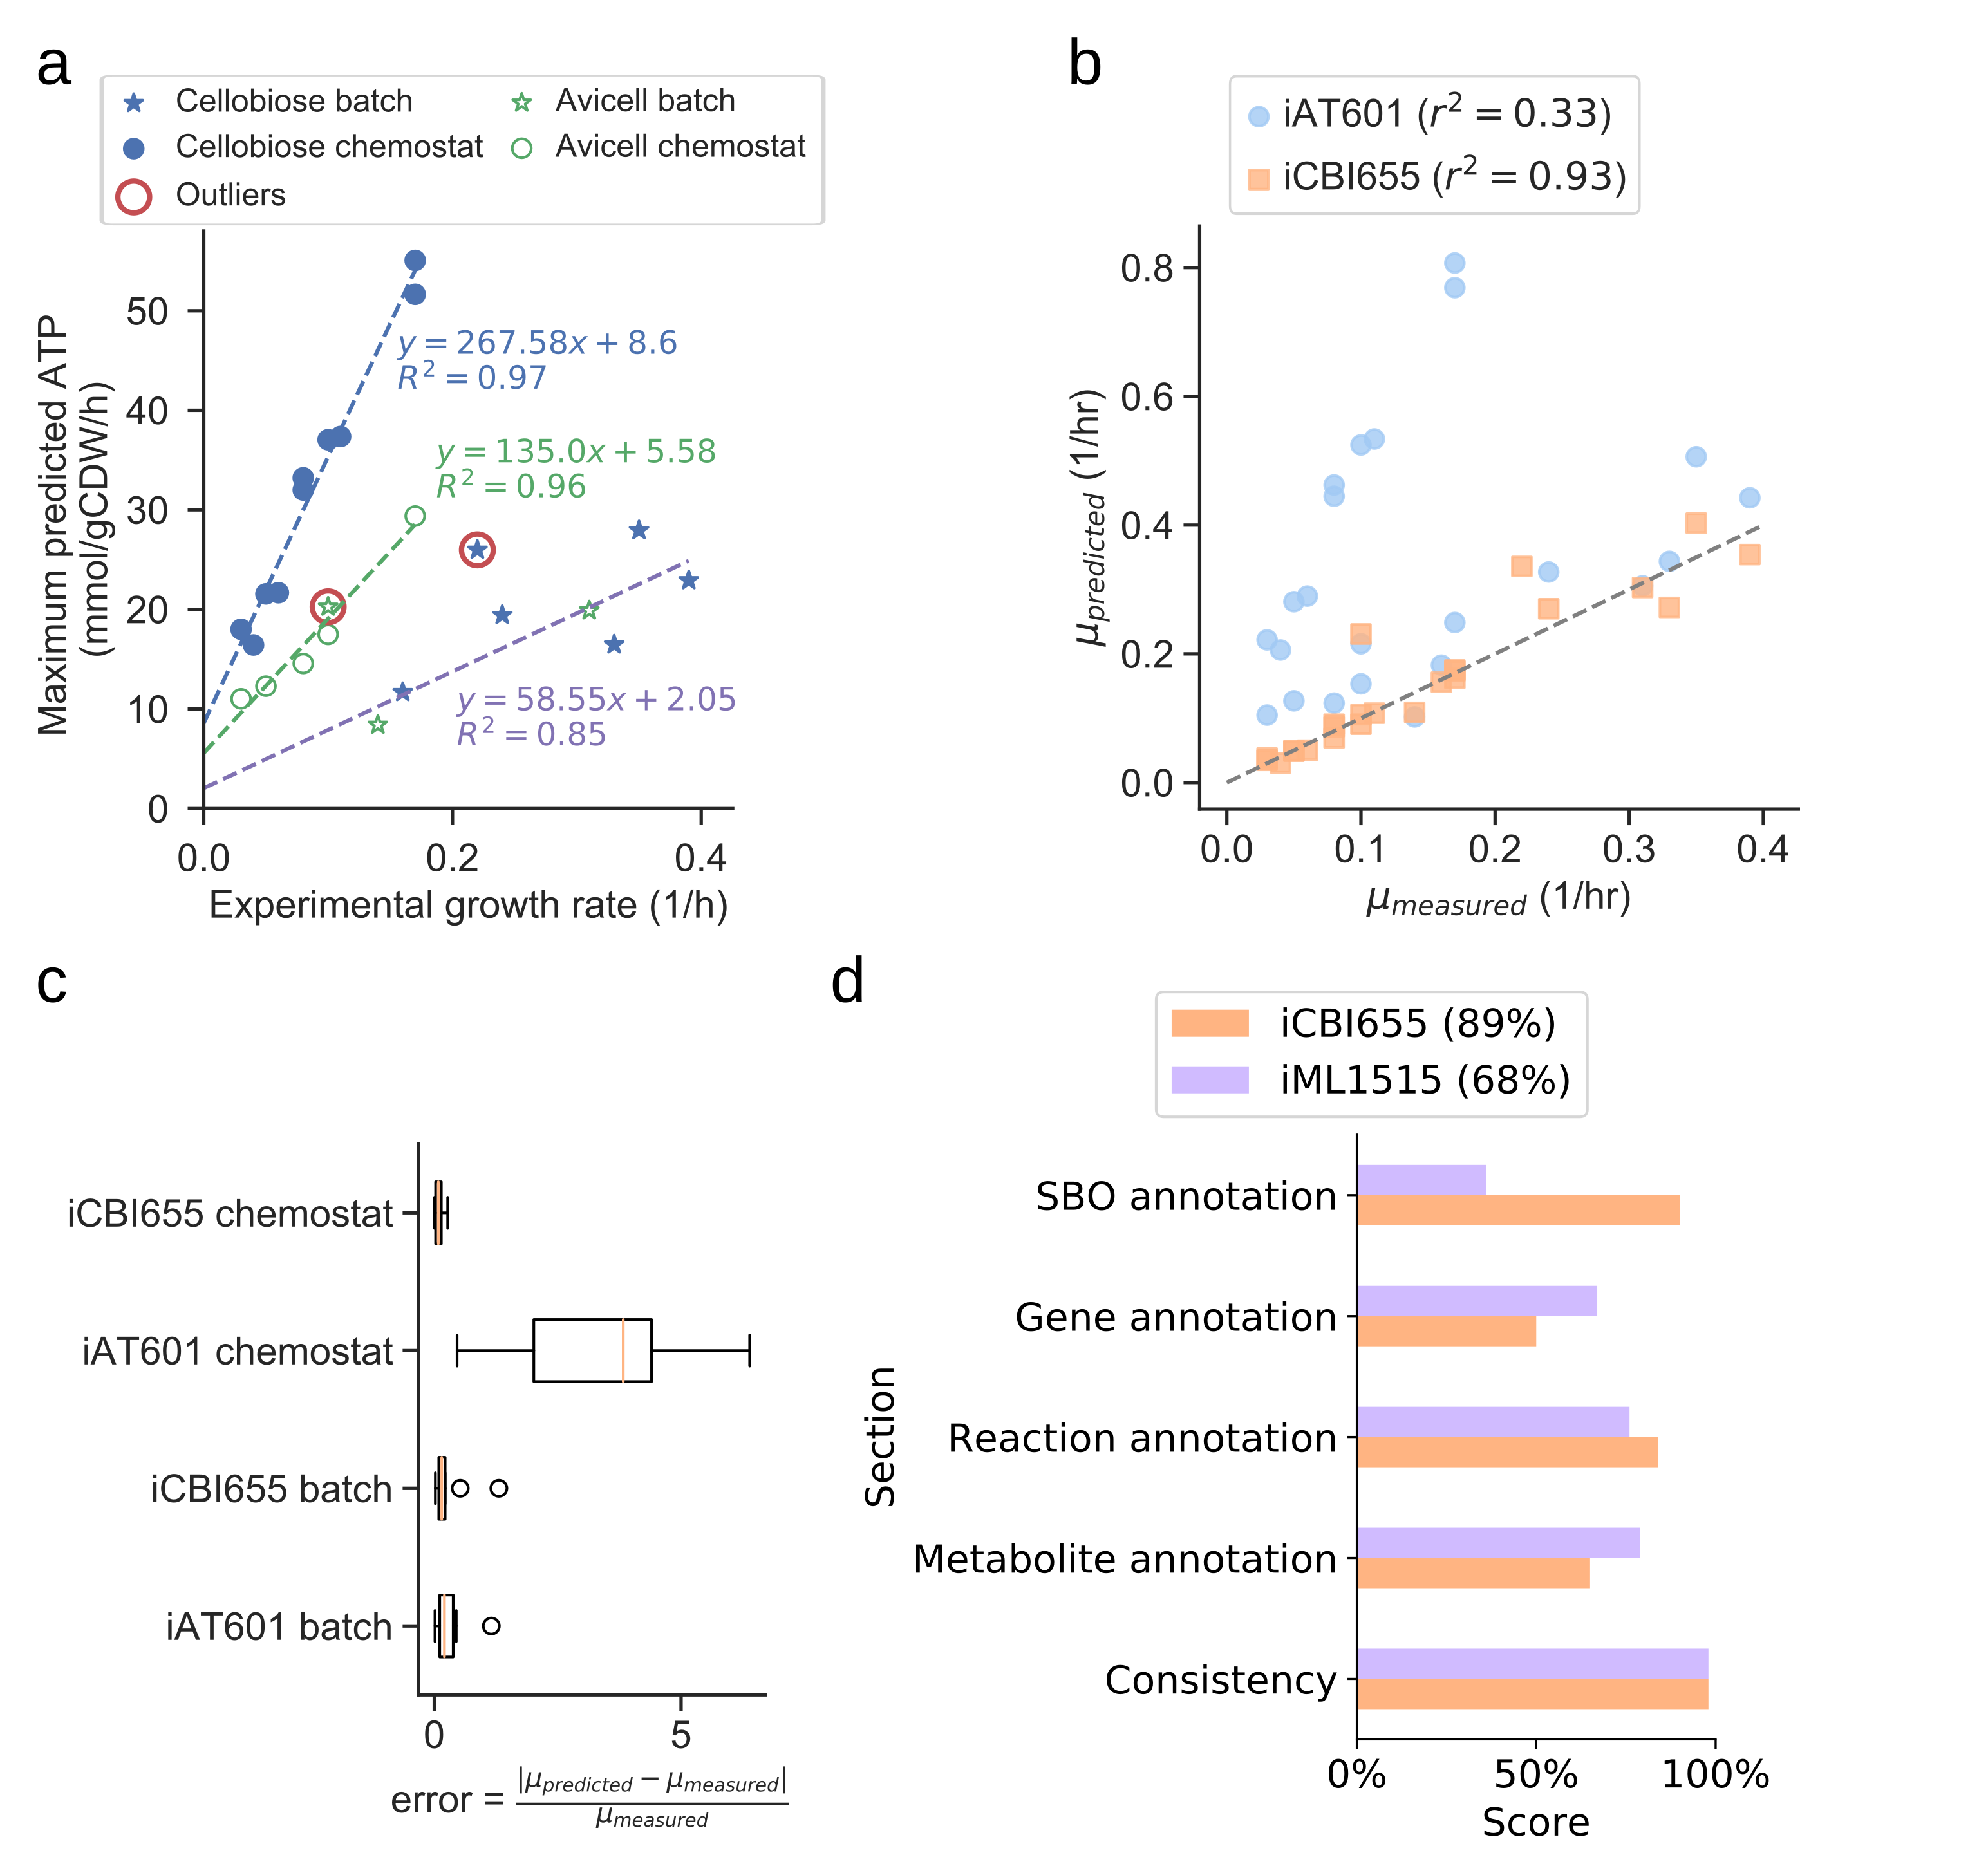
\includegraphics[width=\textwidth,height=\textheight, keepaspectratio]{training.png}
    \caption[Training of iCBI655 model]{%
        (\textbf{a}) Training of GAM and NGAM parameters. Discrete points correspond to experimental data.
    The slope of the linear regression function corresponds to the GAM, while the intercept corresponds to the NGAM.
    The data points circled as outliers were not included in any of the linear regression calculations. (\textbf{b}) Comparison of growth prediction error between iCBI655 and iAT601.
    The measured substrate uptake and product secretion fluxes form each dataset Supplementary Material \ref{sm:datasets} were used to constraint the model and maximum growth rate was calculated.
    $r^2$ corresponds to the Pearson correlation coefficient.
    (\textbf{c}) Error in growth predictions under batch and chemostat conditions.
    Predicted and measured growth rates correspond to the values included in \textbf{b}. (\textbf{d}) Scores provided by the quality control tool Memote\citep{lieven2018} for iCBI655 and iML1515 (overall score indicated in the legend).}
%    %Annotation fields indicate detailed specification of model components critical for model reusability, while the Consistency field verifies biochemical consistency properties such as mass and charge balance of model reactions.}
   \label{fig6:training}
\end{figure}

\subsection{Assessment of model quality and standard compliance with Memote}
The field of metabolic network modeling suffers from a lack standard enforcement and quality control metrics that limits model reproducibility and applicability.
To address this issue, Lieven et al.\ recently developed the Memote framework that systematically test for standards and best practices in GSMs. \citep{lieven2018}
We applied Memote to the iCBI655 model and the \textit{E.~coli} iML1515 model for comparison (Figure~\ref{fig6:training} d). This analysis produces five independent scores that assess model quality.
The \emph{consistency score}  measures basic biochemical requirements, such as mass and charge balance of metabolic reactions, and it was near 100\% for both models.
Additionally, the different annotation scores quantify how many elements in the model contain relevant metadata. More specifically, the \emph{systems biology ontology (SBO) annotation} indicates if an object in the model refers to a metabolite, reaction, or gene; while the respective \emph{annotation scores} of these elements correspond to properties (e.g., name, chemical formula, etc.) and identifiers linking them to relevant databases, e.g., KEGG\citep{kanehisa2000} or modelSEED.\citep{henry2010} The \emph{overall score} is computed as a weighted average of all the individual scores with additional emphasis on the \emph{consistency score}.
In summary, the high scores obtained by iCBI655 reflect the quality of the model and ensures its applicability for future studies.


\subsection{Model-guided systems analysis of proteomics and flux datasets reveals key pathways and cofactors during redox stress} \label{sec:omics_analysis}

% Describe method
Genome-scale models provide a framework to reconcile and analyze multiple datasets at the systems level.
We developed an omics integration method anchored in the quantification of fold change (FC) between case and control samples. FC generalizes to different data types since it is often quantitatively reliable, while more precise metrics like intracellular protein or metabolite concentrations require more sophisticated targeted approaches for quantification. Furthermore, our method does not require one to mechanistically formulate or assume a quantitative relationship between omics measurements and simulated fluxes (Figure~\ref{fig6:proteomics}a).
We first compare simulated flux changes, that are predicted from measured flux changes, against measured omics fold changes.
Then, we identify for further analysis \emph{consistent reactions}, i.e., reactions with fold change of the same sign and different from zero in both measured and simulated fluxes (Section~\ref{sec:proteomics_method}).

\begin{figure}[hp]
    \centering
    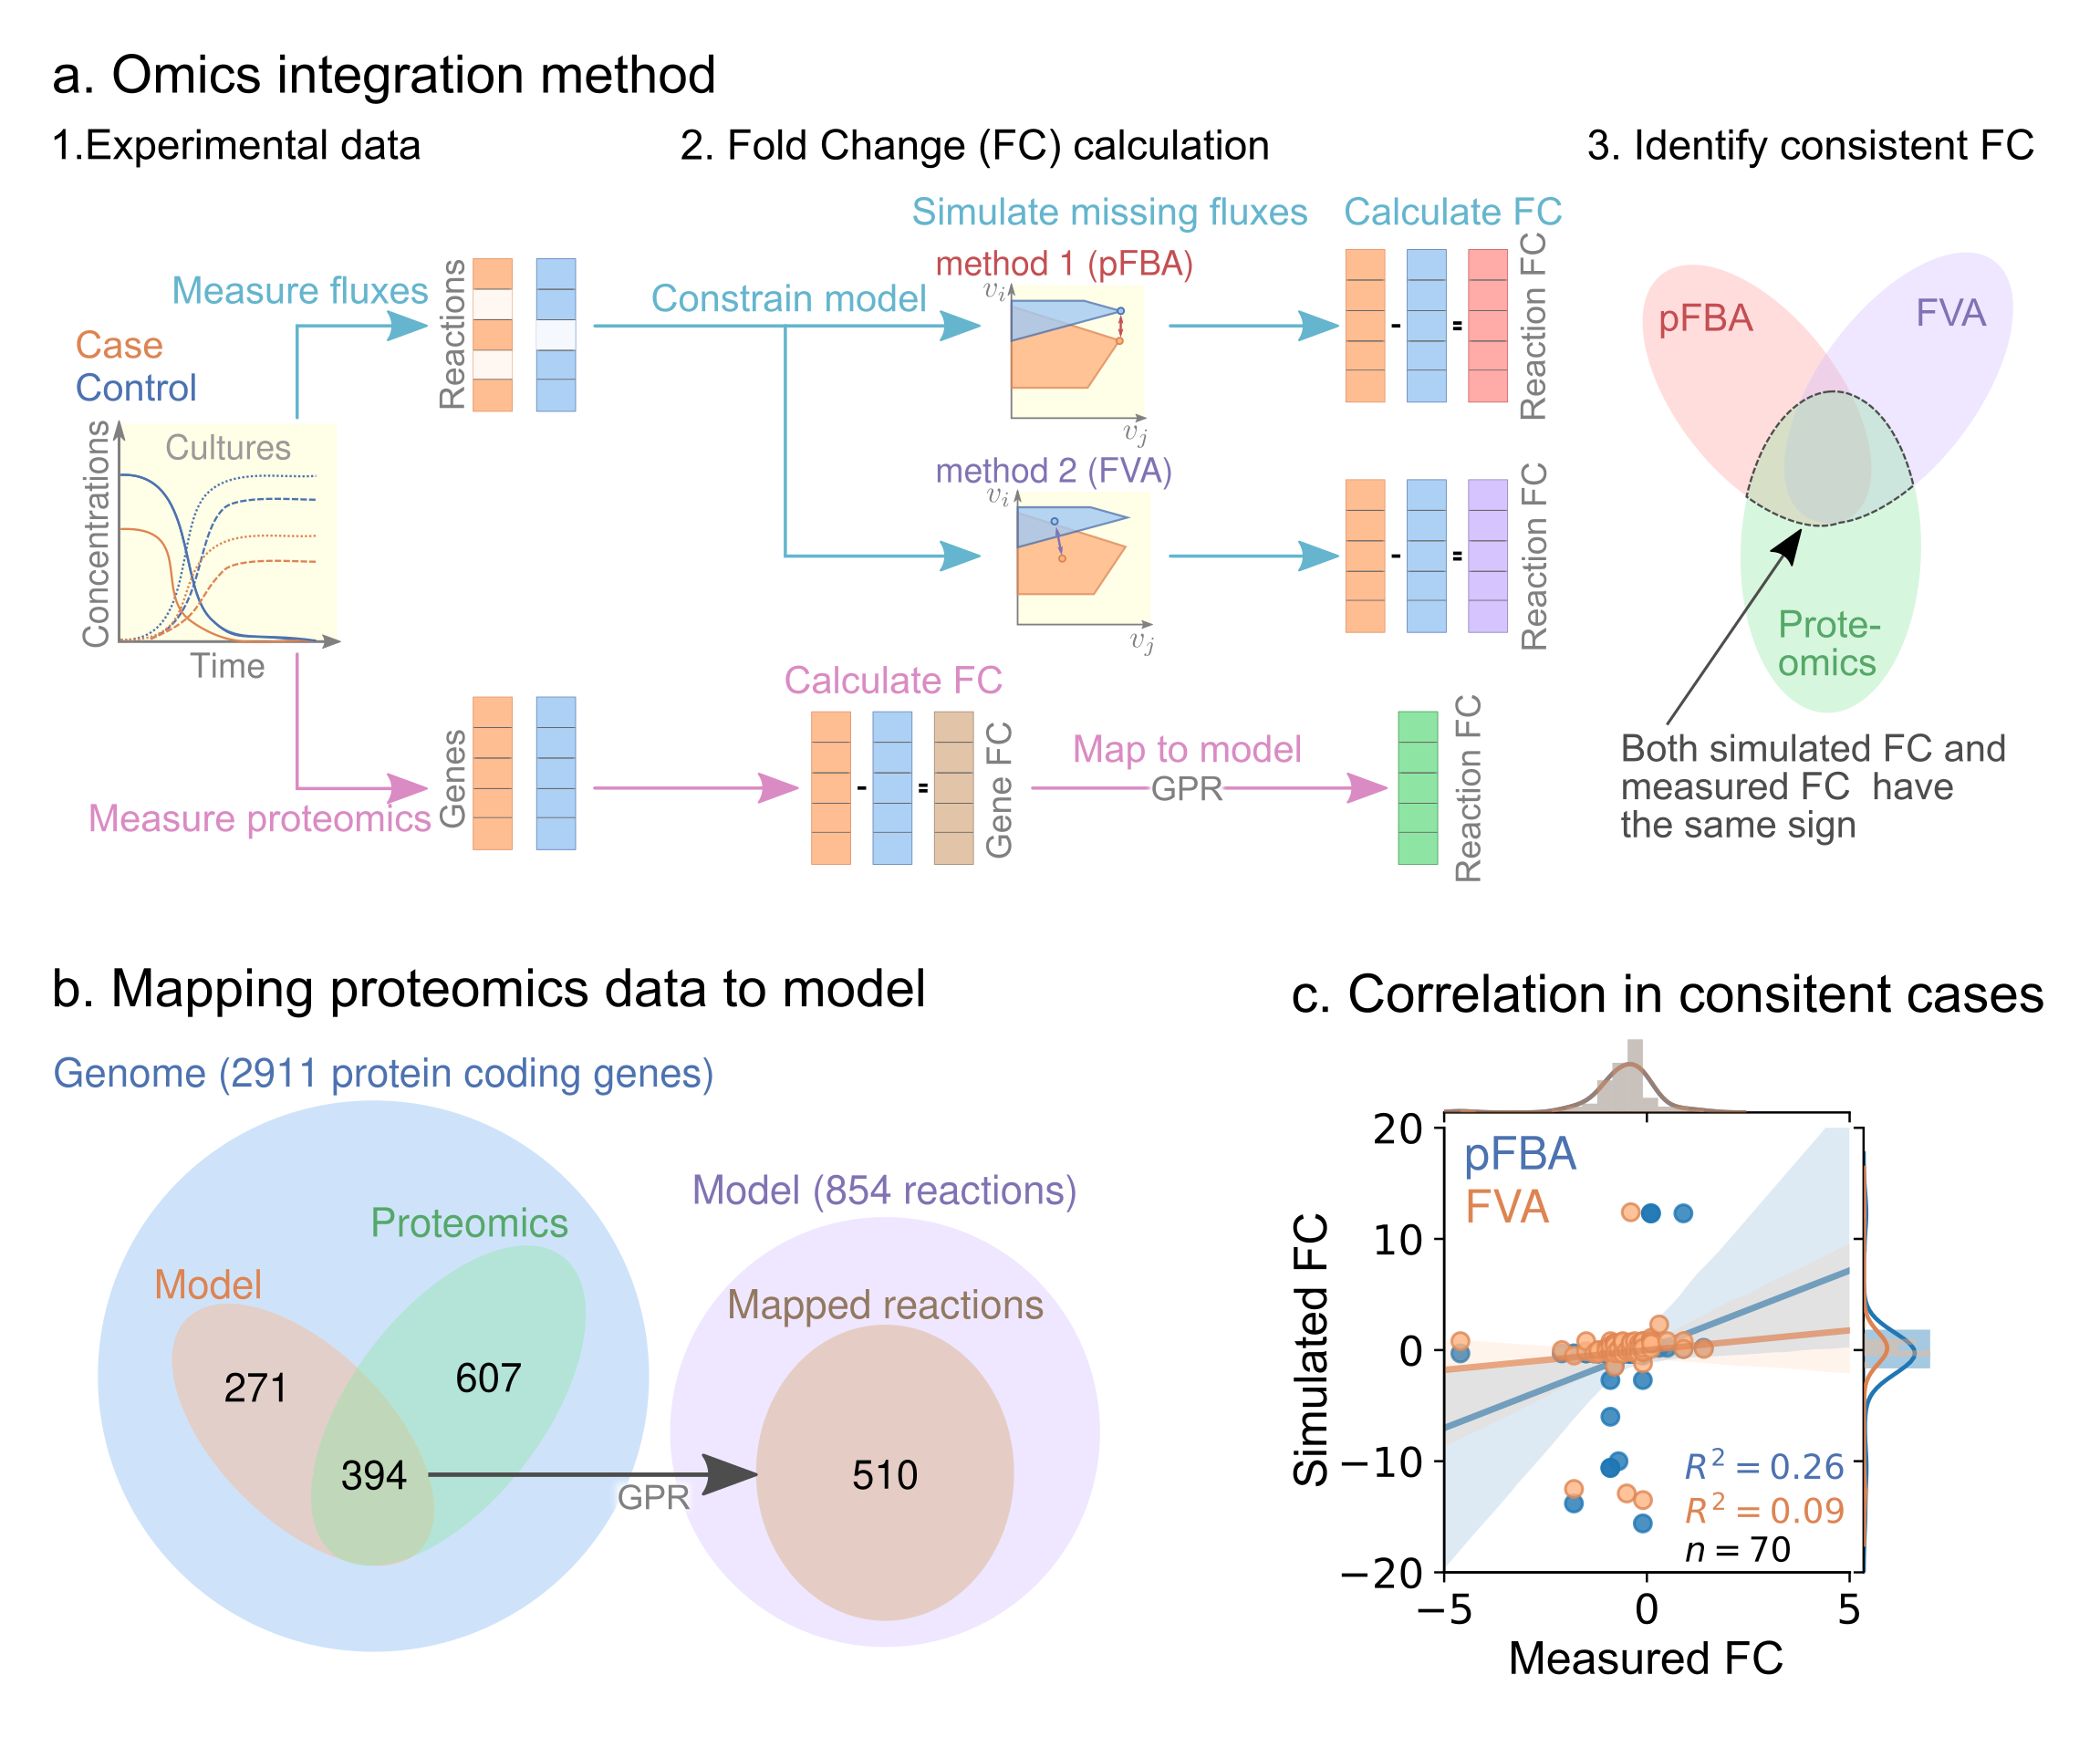
\includegraphics[width=\textwidth, keepaspectratio]{proteomics_method.png}
    \caption[Multi-scale data integration procedure]{(\textbf{a.}) Multi-scale data integration and analysis procedure. (\textbf{b.}) Mapping of proteomics data for the \textit{$\Delta$hydG-$\Delta$ech} case study to model reactions. (\textbf{c.}) Correlation between measured fold changes and simulated fold changes (pFBA in blue and FVA in orange) for all 70 consistent reactions of the \textit{$\Delta$hydG-$\Delta$ech} case study.}
    \label{fig6:proteomics}
\end{figure}

We applied this method to compare the \textit{C.~thermocellum} wild-type against the \ko{hydG,ech} strain. This mutant was engineered to redirect electron flow from hydrogen to ethanol by removal of primary hydrogenases.\citep{biswas2015, thompson2015}
First, we obtained measured FC by mapping the measured proteomics data to 510 out of the 856 reactions in the model thorough the gene-protein-reaction (GPR) associations (Figure~\ref{fig6:proteomics}b).
Then, we identified 70 consistent reactions by comparing measured FC with two types of simulated FC: i) parsimonious flux balance analysis (pFBA) that determines the flux distribution with the lowest total flux and ii) flux variability analysis (FVA), which identifies the feasible flux range of each reaction.
The Pearson correlation coefficients between simulated and measured fluxes for the consistent reactions were 0.26 and 0.09 for pFBA and FVA respectively (Figure~\ref{fig6:proteomics}c).
In general, the FVA reaction flux ranges remained mostly unchanged, suggesting that pFBA is a better representation of actual metabolic fluxes as previously observed.\citep{machado2014}
Consistent reactions where flux and protein fold change have the same sign but different magnitude can be good indicators to identify regulatory effects at the metabolic level, e.g., substrate concentration affecting enzyme saturation ($K_m$), substrate and product concentrations affecting thermodynamic feasibility, and allosteric regulation. Alternatively, these discrepancies between measured and simulated FC magnitude could also be linked to enzyme efficiency ($K_{cat}$), e.g., highly efficient enzymes will have a small concentration increase  but a high flux increase.


The top consistent reactions with the highest proteomics FC magnitude (Supplementary~Material~\ref{sm:figures} - Table~S1) belong primarily to the central metabolism of \textit{C.~thermocellum} (Figure~\ref{fig6:map}a). Central metabolic pathways in this organism have been studied in depth with the aim of increasing ethanol production. We will provide a brief overview of the most recent findings and compare them with the results obtained from our analysis.

\begin{figure}[p]
    \centering
    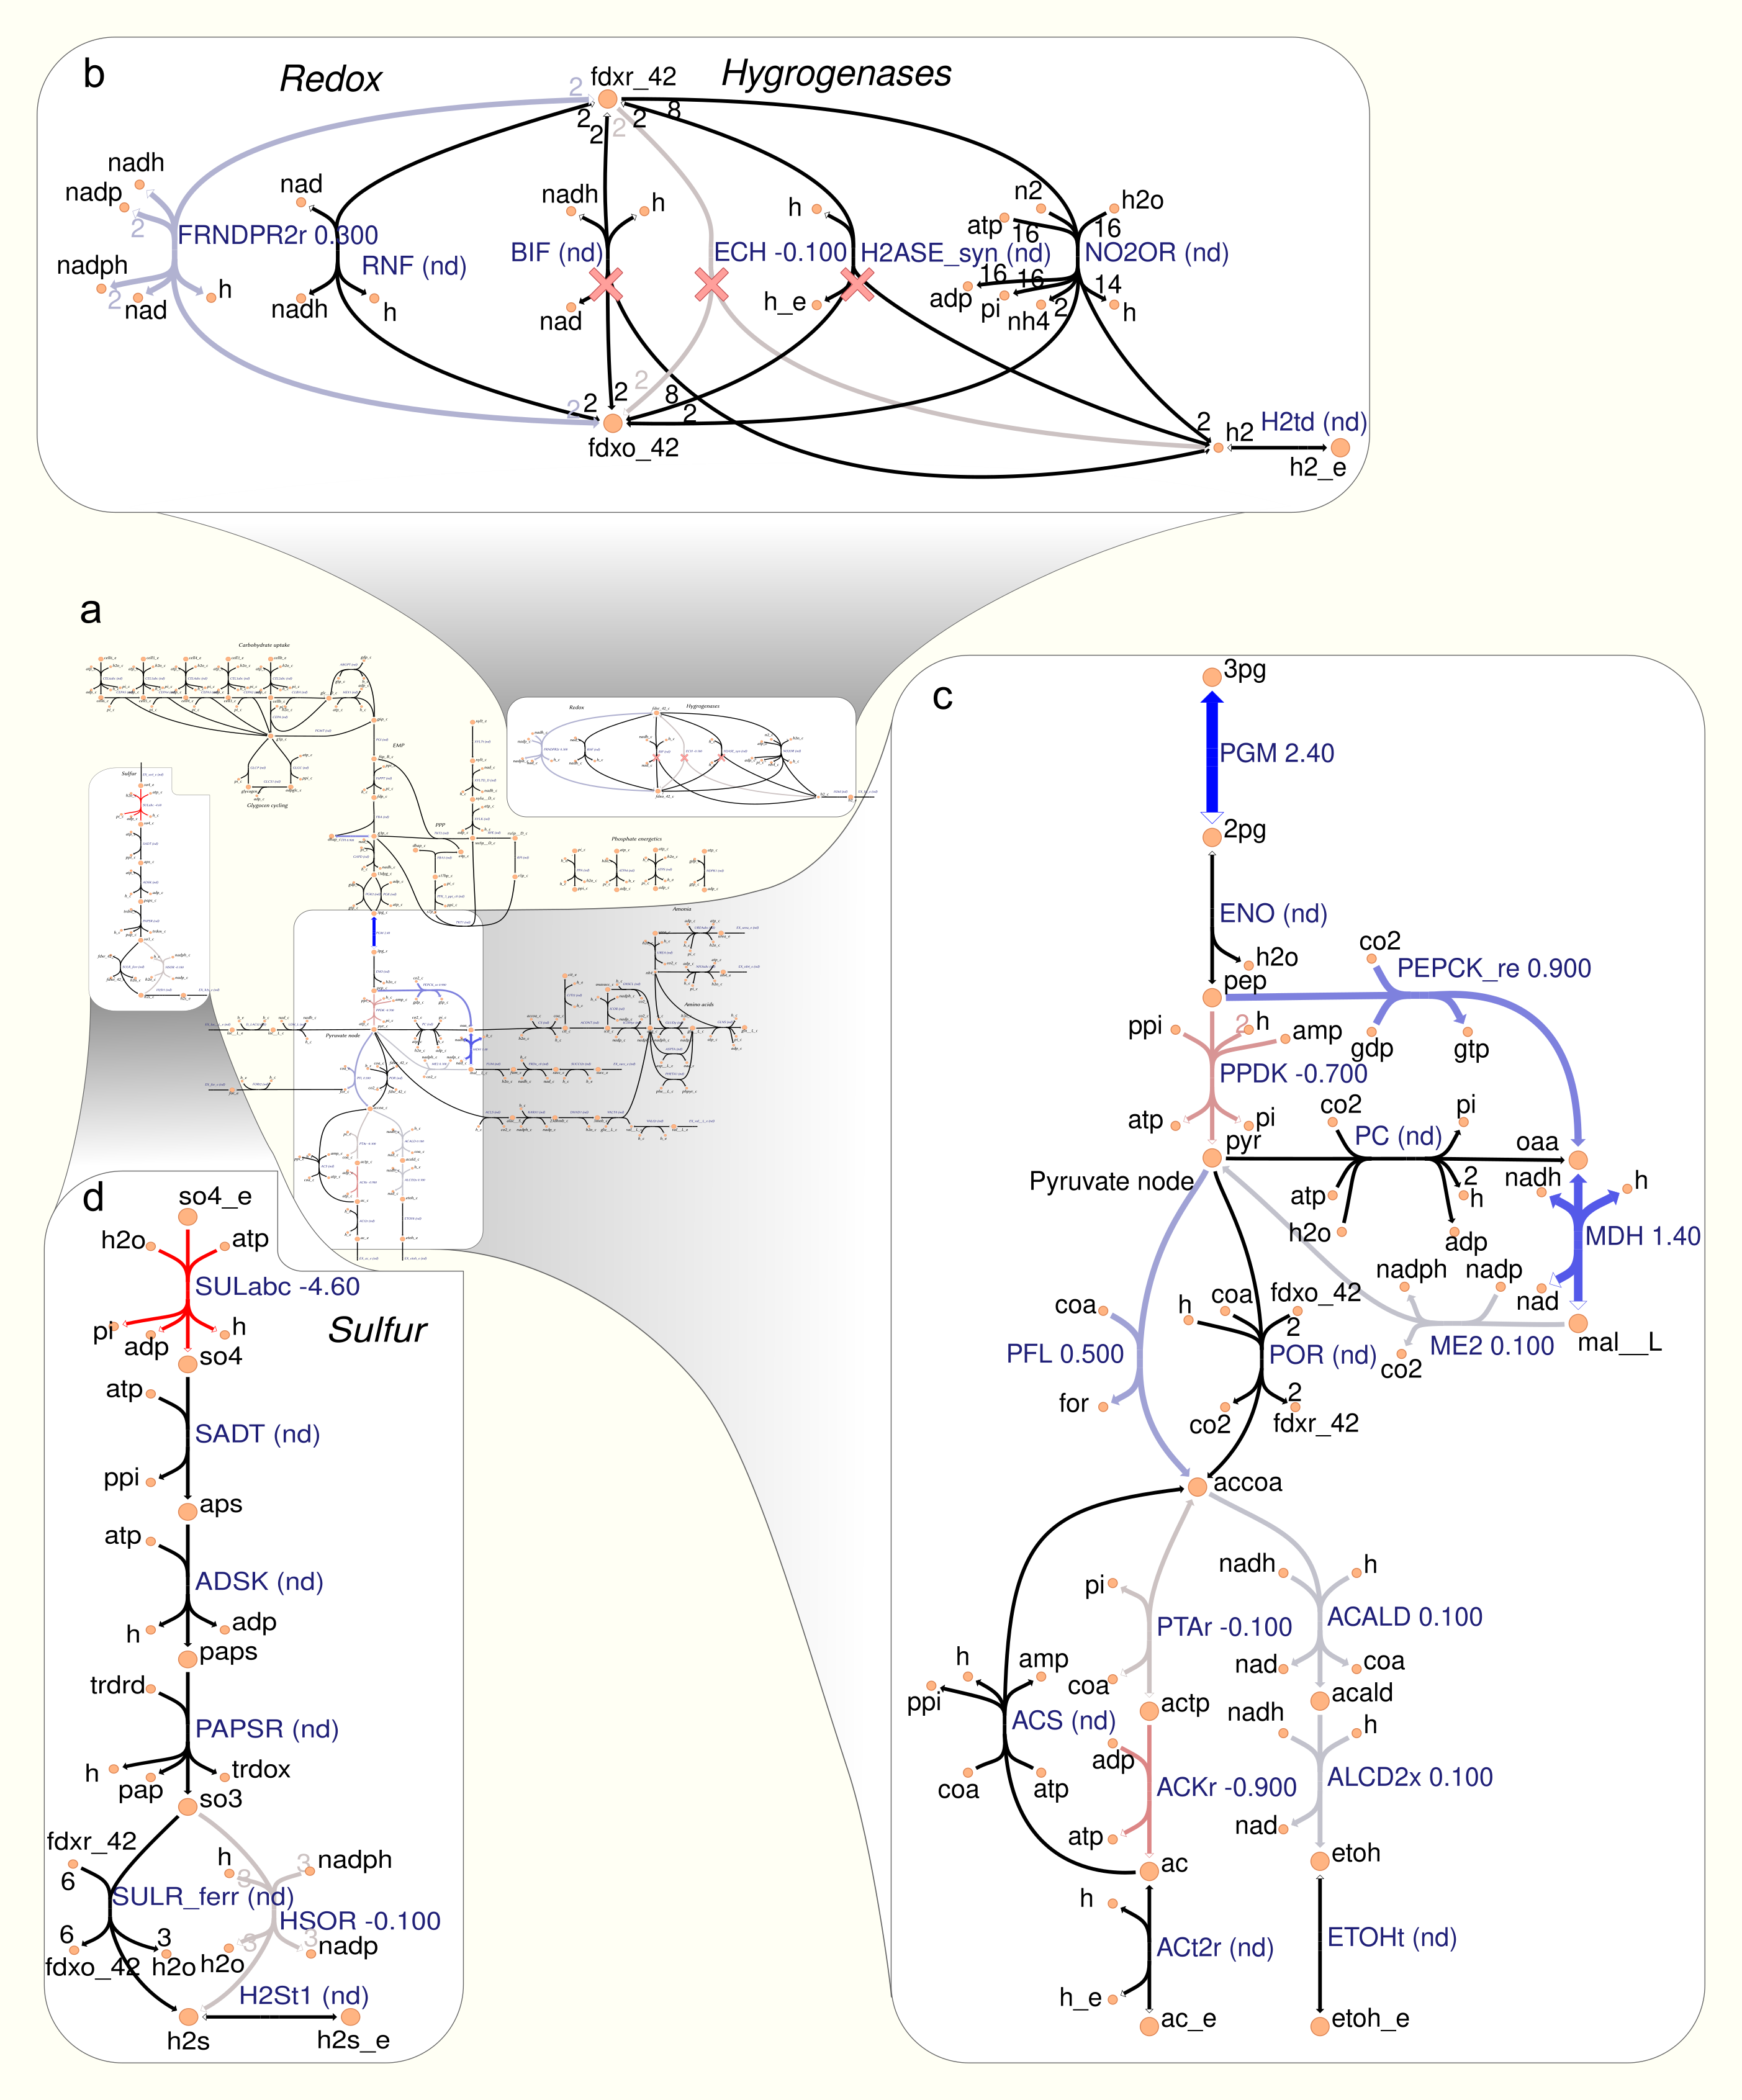
\includegraphics[width=0.91\textwidth, keepaspectratio]{proteomics_fc_map.png}
    \caption[Metabolic map visualization of proteomics data]{Metabolic map visualization using the iCBI Escher map. Values next to reaction labels correspond to proteomics fold change between \textit{$\Delta$hydG-$\Delta$ech} and wild-type strains only for the 70 consistent reactions identified by the omics analysis (Section \ref{sec:omics_analysis}). Reaction line thickness and color intensity are proportional to the fold change values, except for reactions drawn in black which do not belong to the 70 consistent reactions. A gradient from gray to blue is used to indicate a positive flux increase, while a gradient from gray to red is used to indicate a negative flux increase. Note that the positive or negative signs only indicate the directionality of reversible reactions. (\textbf{a.}) Overall map of central metabolism. (\textbf{b.}) Redox and hydrogenase metabolism, reactions marked with a red cross are deleted in \textit{$\Delta$hydG-$\Delta$ech}. (\textbf{c.}) Pyruvate metabolism. (\textbf{d.}) Sulfur metabolism.}
    \label{fig6:map}
\end{figure}

\paragraph{Redox metabolism}
\textit{C.~thermocellum} has various reactions to regulate the relative concentrations of NADH, NADPH, and Reduced ferredoxin (Figure~\ref{fig6:map}b), since these cofactors are used as electron donors with high specificity throughout metabolism. Additionally, several hydrogenases oxidize these reduced cofactors to molecular hydrogen that is secreted by the cell to maintain redox balance. Removal of these hydrogenases through deletion of \textit{ech} (corresponding to the ECH reaction) and \textit{hydG} (corresponding to the BIF and H2ASE\_syn reactions) was successfully applied to increase ethanol yield.\citep{biswas2015}
Thompson et al.\citep{thompson2015}\ characterized the \ko{hydG,ech} strain in depth by analysis of its extracellular fluxes with a core metabolic model, concluding that the major driver for ethanol production was redox balancing rather than carbon balancing. To overcome the predicted production bottlenecks in redox metabolism, \textit{nfn} (corresponding to the  FRNDPR2r reaction) and \textit{rnf} (corresponding to RNF) over-expression were suggested.
In a subsequent study, Lo et al.\citep{lo2017}\ successfully over-expressed \textit{rnf} in \ko{hydG,ech}, but that did not lead to increase in ethanol yield. However, deletion of \textit{rnf} and \textit{nfn} led to lower ethanol and increase hydrogen production in \ko{hydG}. This suggests that while the \textit{rnf} and \textit{nfn} enzymes are essential for ethanol production, they do not constitute the primary bottlenecks in this pathway.

\paragraph{Pyruvate node and the malate shunt}
Deng et al.\citep{deng2013}\ investigated the importance of the malate shunt in \textit{C.~thermocellum}, which converts phosphoenolpyruvate (\textit{pep}) to oxaloacetate (\textit{oaa}) and then to pyruvate (\textit{pyr}), while transforming one mol of NADH generated during glycolysis to a mole of NADPH (Figure~\ref{fig6:map}c). Interestingly, the authors noted that replacement of the malate shunt by alternative pathways not linked to NADPH increased ethanol production, carbon recovery, and reduced amino acid formation, suggesting that NADPH can be oxidized by secondary pathways.
% SG: Remove the part below because the interpretation might be limited to ethanol pathways but not applicable at the cellular level:
%A recent study \citep{dash2019} of ethanol production pathways predicted that the thermodynamic feasibility of the malate shunt can be highly dependent on pH and the concentration of associated metabolites, in particular CO$_2$ concentrations, which was linked to the enhanced growth rates of \textit{C.~thermocellum} under CO$_2$ supplementation.\citep{xiong2016} If CO$_2$ activates the malate shunt, that would imply this pathway is more efficient for cell growth.
%\singlespace
%\todo[inline]{ Regarding the hypothesis of the malate shunt being more efficient for growth: In deng2013 Fig 2 A they see increased growth rate for me-mdh knockout, but they only have one point in the exponential growth phase. In any case, to test the hypothesis would require co2 supplementation + me-mdh knockout. I suspect the pathway is not necessary more efficient}
%\doublespace

\paragraph{Sulfur metabolism}
Sulfate serves as an electron acceptor to \textit{C.~thermocellum} which is capable of oxidizing it to sulfite and then sulfide (Figure~\ref{fig6:map}d).
Thompson et al.\citep{thompson2015}\ demonstrated that the strain \ko{hydG,ech,pfl}, which cannot grow in conventional medium due to its inability to secrete hydrogen or formate, recovered growth by sulfate supplementation to the culture medium.
More recently, Biswas et al.\citep{biswas2017}\ reported an increase in final sulfide concentration and over-expression of the associated sulfate uptake and reduction pathway in the \ko{hydG} strain, but did not observe a significant difference in final sulfide concentration in \ko{hydG,ech}.
Remarkably, neither of the strains consumed cysteine from the medium, unlike the wild-type.
Sulfide can be converted to cysteine by CYSS (Cysteine synthase) or homocysteine and then methionine by SHSL2 and METS (succinyl-homoserine succinate-lyase and methionine synthase), but the connection between the cessation of cysteine uptake and sulfate metabolism remains unclear.


\paragraph{Proteomics data reveals the importance of NADPH}
Our analysis reveals consistent indications of increased NADPH biosynthesis in the \ko{hydG,ech} mutant across three major metabolic areas: i) an increased translation of FRNDPR2r (also known as NFN) that converts one mol of reduced ferredoxin (\textit{fdxr\_42}) and one mole of NADH into two moles of NADPH.
(Figure~\ref{fig6:map}a);
ii) increased translation of all three malate shunt enzymes and decreased translation of the alternative route PPDK; %(Figure~\ref{fig6:map}b});
and iii) decreased translation of sulfur transporter and of HSOR that oxidizes sulfite into sulfide consuming NADPH.
These observations are consistent with the failure of \textit{rnf} over-expression to enhance ethanol production\citep{lo2017}, since RNF produces NADH but the key cofactor bottleneck seems to be NADPH. Furthermore, a direct look at the proteomics data revealed that RNF subunits (Clo1313\_0061-Clo1313\_0066) had a statistically significant translation decrease in the mutant (Supplementary Material \ref{sm:datasets}).
The preference of \ko{hydG,ech} towards NADPH could be due to the cofactor specificity of the remaining redox balancing pathways (e.g., isobutanol), thermodynamics and protein cost constraints, or a combination of both. A recent analysis of the thermodynamics of ethanol production in \textit{C.thermocellum} that did not include peripheral pathways highlighted the importance of engineering strategies based on NADPH (e.g., introduction of NADPH-linked GAPDH (that converts glyceraldehyde-3-phosphate to 3-phospho-D-glyceroyl phosphate during glycolysis, and NADPH-FNOR that transfers electrons from reduced ferredoxin to NADPH.


\paragraph{Analysis of simulated fluxes to predict the function of NADPH}
The analysis based on consistent reactions strongly indicates that NADPH production is important in the mutant to achieve redox balance.
However, since not all reactions in the model could be mapped to proteomics measurements and carbon recovery was lower in the mutant strain,\citep{thompson2015} it remains to be fully clarified where NADPH is being oxidized.
The flux simulations used to identify consistent reactions take into account all metabolic reactions.
Thus, we examined the remaining reactions that had different fluxes between wild-type and mutant, and limited this search to exchange reactions and reactions that involve NADPH (Supplementary Material \ref{sm:figures} - Table S2).
These simulated fluxes predicted an increase in the isobutanol pathway, including keto-acid reductoisomerase (KARA1) that consumes NADPH and isobutanol secretion (EX\_ibutoh\_e).
The isobutanol pathway can consume NADPH through several enzymes\citep{lin2015} and has increased flux during overflow metabolism at high-substrate loading.\citep{holwerda2014,thompson2017}
The model also predicted a decrease in valine secretion (EX\_val\_\_L\_e), since the isobutanol pathway competes with the valine pathway after KARA1.
Remarkably, this prediction is consistent with the lower valine secretion measured in \ko{hydg,ech}.\citep{biswas2017} %by Biswas et al.\ (This finding is not discussed in main text, see Supplementary Fig. S2 in their study).
Note that a certain amount of NADPH is likely oxidized by the mutated alcohol-dehydrogenase enzyme observed after short adaptation in \ko{hydG} that is compatible with both NADH and NADPH,\citep{biswas2015} but this feature is not captured by the model since in general gene knockouts are simulated by blocking the associated reactions.
Overall this analysis indicates that \ko{hydg,ech} likely increases isobutanol secretion to alleviate redox imbalance.

\paragraph{Summary}
Previous studies of \ko{hydg,ech} that used secretion fluxes\citep{thompson2015} or omics\citep{biswas2017} independently pointed at the general presence of redox imbalance in this mutant but were not able to resolve the specific importance of NADPH and associated pathways identified here through dataset integration with the genome-scale model. This illustrates the power of the model as contextualization tool, and provides new insights into the redox bottlenecks present in \textit{C.~thermocellum} that are critical in the production of reduced molecules. The reactions with major translational changes identified here can serve as the targets for further engineering.


\section{Model-guided design of platform strains for biofuel production}

% Context and explanation
Another common application of genome-scale models is strain design. \citep{long2015, ng2015, maranas2016, wang2018, garcia2019, garcia2019b, garcia2019c}
We used the iCBI655 model combined with the ModCell tool\citep{garcia2020b} to design \textit{C.~thermocellum} platform strains for production of alcohols and esters.
Briefly, the modular cell design problem formulation is as follows: We aim to build a strain that when combined with different pathway modules it will lead to production strains that display a target phenotype, in this case growth-coupled to product synthesis. Quantitatively, this phenotype is defined as weak growth coupled to product formation (\textit{wGCP}) and it corresponds to the minimum product synthesis rate at the maximum growth rate.
The design variables to attain the target phenotypes correspond to genetic manipulations of two types: i) reaction deletions, limited by the parameter $\alpha$, that correspond to gene knock-outs; and ii) module reactions, limited by the parameter $\beta$, that correspond to reactions deleted in the chassis but added back to specific modules enhancing the compatibility of the modular cell. Once these two parameters are specified, the solution to the problem is a set of Pareto optimal designs named Pareto front. In a Pareto optimal design the performance (i.e., objective value) of a given module can only be increased at the expense of lowering the performance of another module.
To characterize the practicallity of each design, we say it is compatible with certain modules if the design objective is above a specific threshold (0.5 in this study). Hence, the \emph{compatibility} of a design corresponds to the number of compatible modules.

% Results
To design \textit{C.~thermocellum} modular cells, we first evaluated a range of design parameters $\alpha$ and $\beta$ with an increasing number of genetic manipulations (Figure~\ref{fig6:designs} a).
As expected, increasing the number of deletions leads to more compatible designs, at the expense of more complexity in the implementation.
We selected an intermediate point of $\alpha=6, \beta=1$ for further analysis.
This Pareto front is composed of 12 designs that cluster into two groups (Figure~\ref{fig6:designs} b).
The first group (e.g., designs 8, 3, and 9) are compatible to all products except butanol and its derived esters, whereas the second group (e.g., 2, 12, 1, 10) emphasizes high objective value in butanol and its derived esters.
To understand the characteristics of each group we can inspect the deletions of each design (Figure~\ref{fig6:designs} c).
Designs 8, 3, and 9 all have in common H2ASE\_syn, GLUDy (NADPH-dependent Glutamate dehydrogenase), PPDK, and FRNDPR2r deletion, while the last two deletions never appear in 2, 12, 1, or 10. % NOTE: All reaction abbreviations except GLUDY are noted earlier
The majority of deletion targets are central metabolic reactions (Supplementary Material \ref{sm:figures} - Table S3).
These include common targets, such as hydrogenases (e.g., the cluster of designs 10, 12, 4, 11, 2, and 7 all contain the \ko{hydg,ech} genotype discussed earlier), or the removal of reactions that form fermentative byproducts such as ALCD2x and ACALD (ethanol), PFL (formate), LDH\_L (lactate).
Interestingly ACKr or PTA (acetate) do not appear in this list, likely because acetate production can serve as a regulatory valve for redox metabolism, in particular in a platform strain that must be compatible with products of diverse degree of reduction.
More interestingly, we also find important branch-point reactions\citep{stephanopoulos1991} in central metabolism as deletions that have not been explored in the context of strain design.
%,likely since they do not present an immediate connection to electron and carbon fluxes, and hence require a more systematic framework to be identified.
Most prominently, these include GLUDy, PEPCK\_re, and PPDK, which appear in 50\%, 33\%, and 25\% of the designs, respectively
(Supplementary Material \ref{sm:figures} - Table S3).
Both PEPCK\_re and PPDK present two alternative routes that influence the ratio of NADPH to NADH, which is relevant to control metabolic fluxes though the specific dependencies of certain enzymes towards each redox cofactor.
GLUDy consumes NADPH and is a key reaction in amino-acid metabolism, hence this enzyme and related ones (e.g., GLUSy: NADPH-dependent Glutamate synthase) are interesting targets for practical implementation.

Two representative designs from the groups mentioned earlier are 12 and 3.
Their feasible growth and production phenotypes reveal a tight coupling between product formation and growth rate (Figure~\ref{fig6:designs} d).
This phenotype enables pathway optimization through adaptive laboratory evolution, as previously done for ethanol,\citep{tian2016} overcoming one of the main challenges of \textit{C. thermocellum} engineering that is optimization of enzyme expression levels. Hence, the proposed chassis strains can also serve as platforms for pathway selection and optimization.
In summary, this analysis demonstrates the potential of the model to identify non-intuitive metabolic engineering strategies that can be key to build effective modular platform strains for the production of biofuels and biochemicals in \textit{C. thermocellum}.

\begin{figure}[hp]
    \centering
    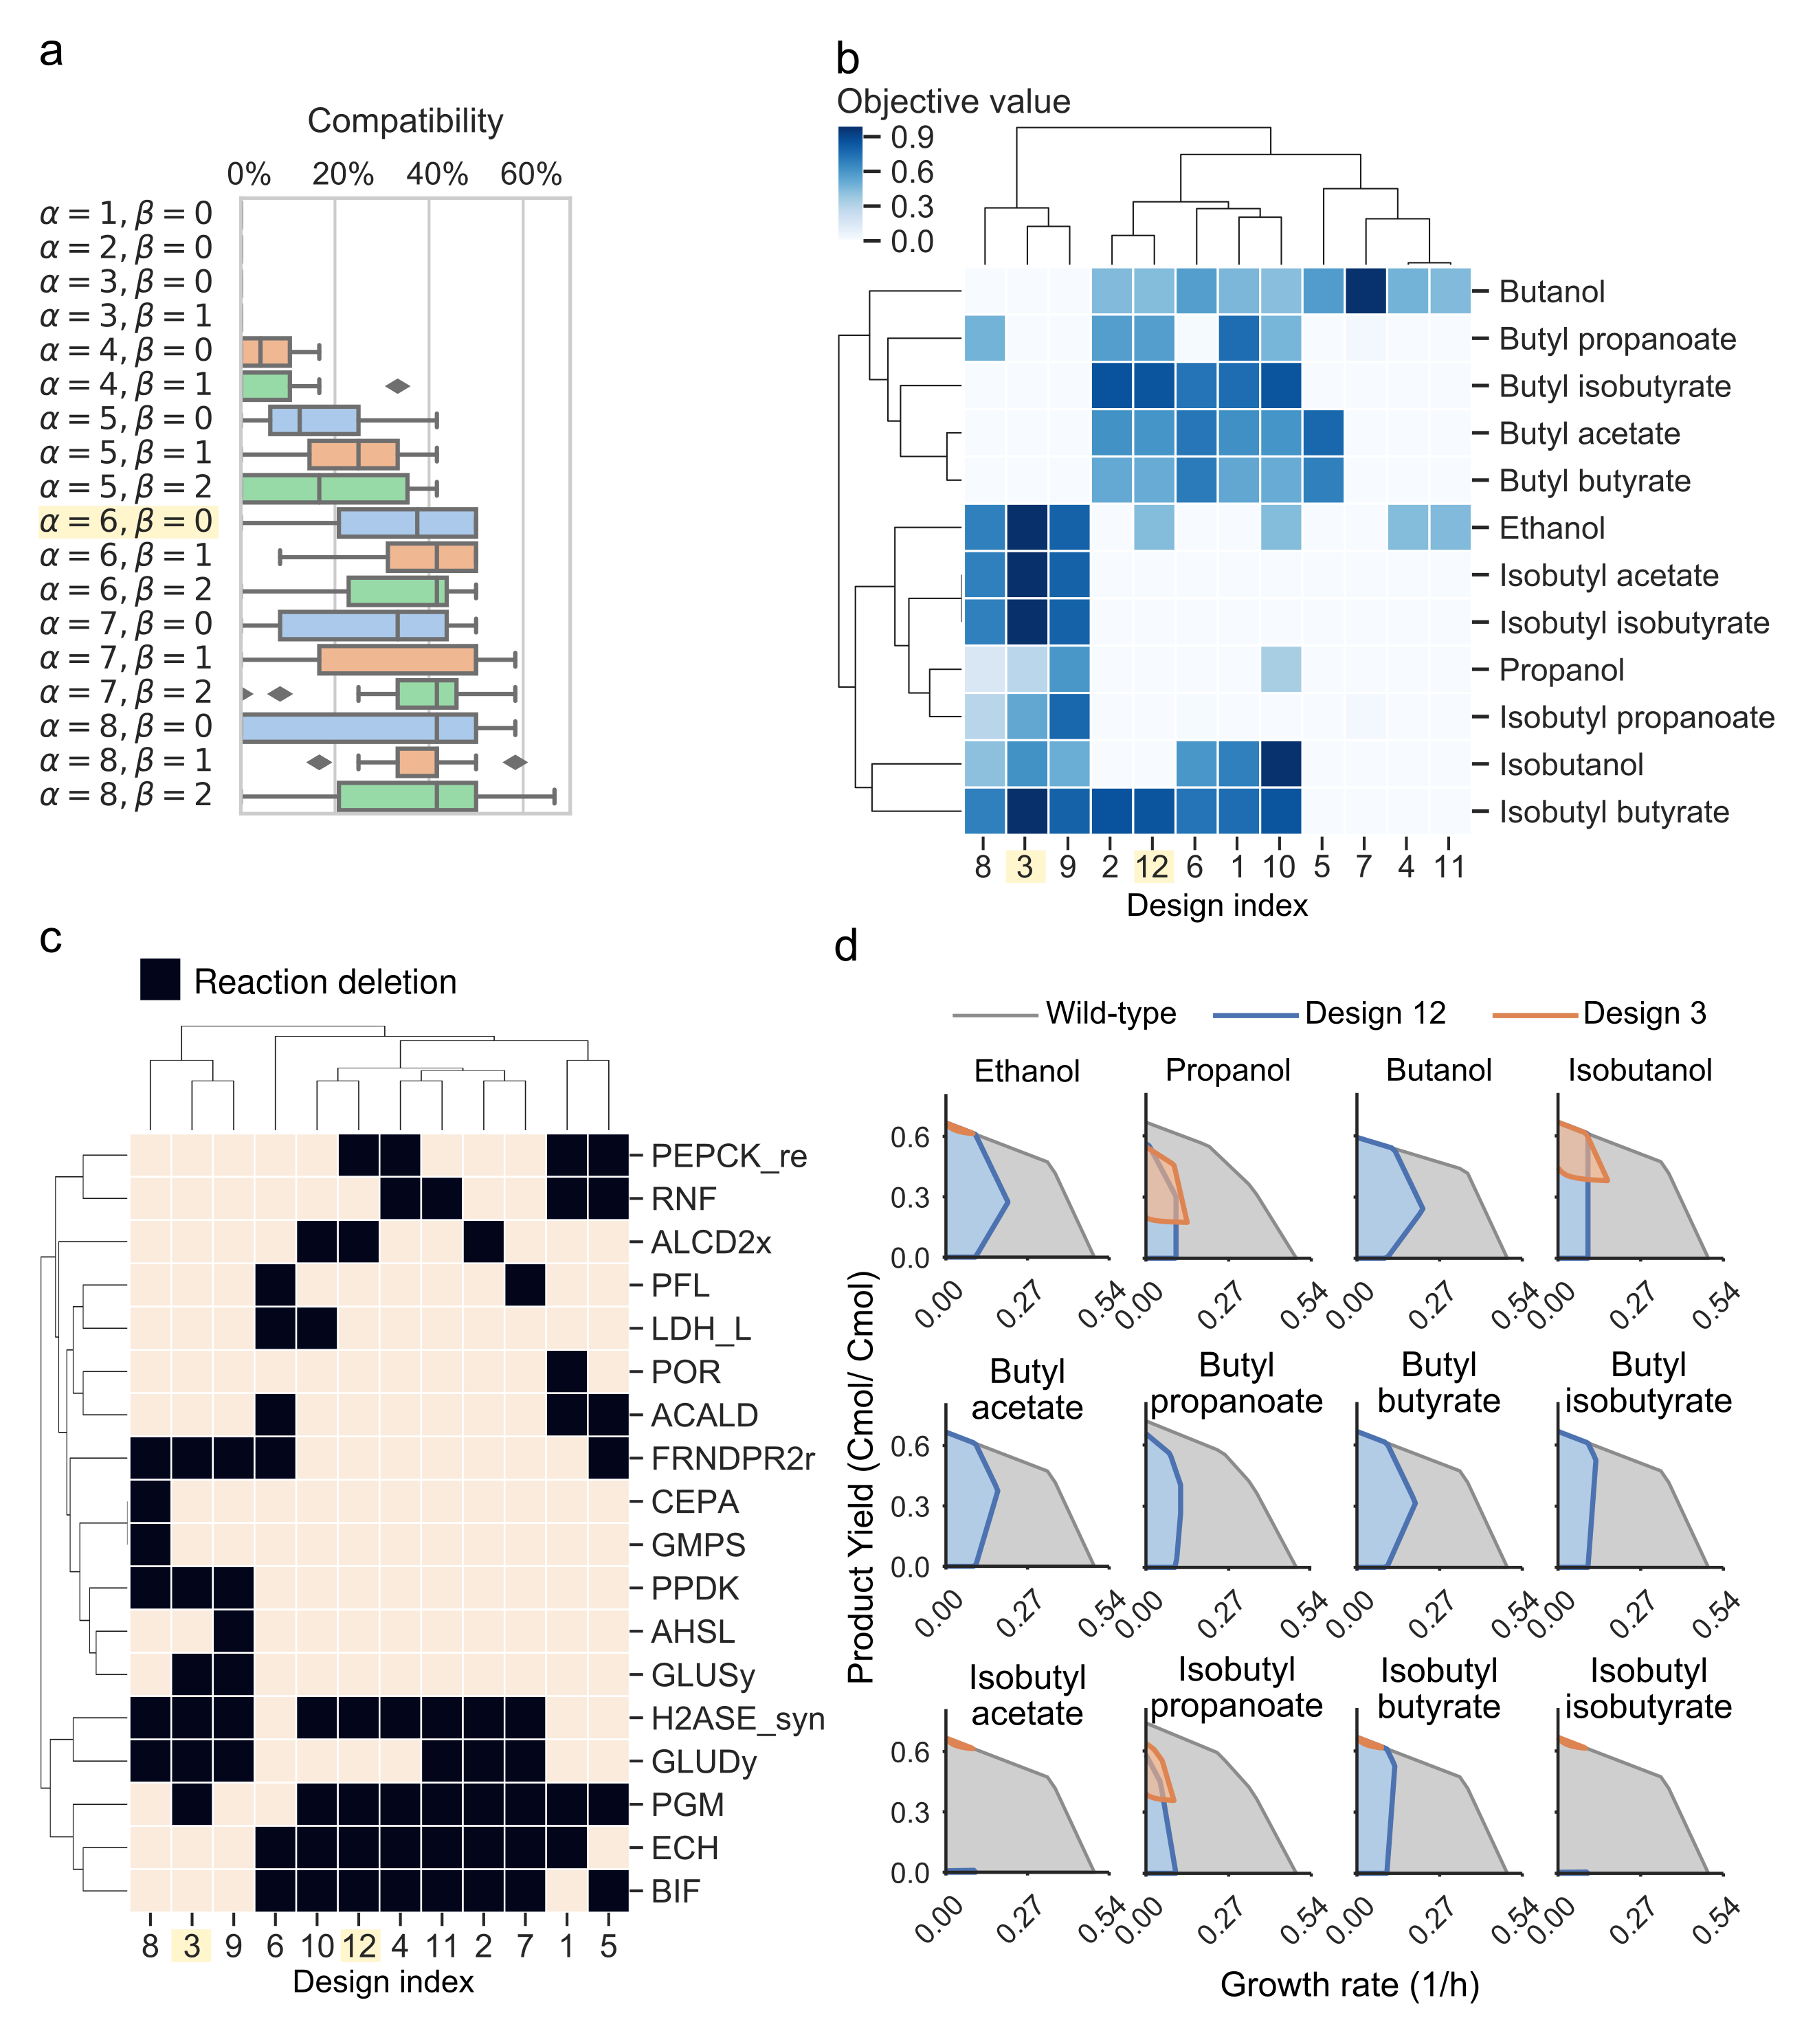
\includegraphics[width=0.95\textwidth, keepaspectratio]{designs.png}
    \caption{Proposed modular cell designs for a \protect\textit{C. thermocellum} platform and 12 alcohols and esters. (\textbf{a}) Parameter scan, and compatibility distribution of the designs in each resulting Pareto front. (\textbf{b}) Pareto front for parameters $\alpha=6,\beta=0$. (\textbf{c}) Pareto set for parameters $\alpha=6,\beta=0$. Reaction names and formulas are included in Supplementary Material \ref{sm:figures} - Table S3. (\textbf{d}) Feasible phenotypic spaces according to reaction stoichiometry for selected designs.}
   \label{fig6:designs}
\end{figure}

\section{Conclusions}
In this study we developed a genome-scale metabolic model of the biotechnologically relevant organism \textit{C.~thermocellum}.
Model development followed standards and best practices to ensure reproducibility and accessibility.
We demonstrated the enhanced predictive capacity of the model for diverse fermentation conditions and for the lethality of important mutants.
Genome-scale models have a broad range of applications in systems biology, including metabolic engineering, physiological discovery, phenotype interpretation, and studies of evolutionary processes. \citep{feist2008, palsson2015} To illustrate the model applications, we chose to tackle the challenge of disparate data integration and interpretation at the systems level. We developed a novel method for this purpose, and used it to identify routes in central metabolism that were selected to increase NADPH generation in the \ko{hydg,ech} strain, revealing the importance of this cofactor over its alternatives and providing new engineering targets for enhanced biosynthesis of reduced products in \textit{C.~thermocellum}.
We also illustrated the use of the model to design platform strains, using the ModCell tool.\citep{garcia2019b} The proposed designs cover C2 through C4 alcohols and their derived esters, which are key target molecules for renewable production with \textit{C. thermocellum}.\citep{peters2018}
The proposed designs feature a combination of previously-explored and novel strategies to couple target metabolite production to cellular growth.
The microorganisms \textit{Escherichia~coli} and \textit{Saccharomyces~cerevisiae} are two major workhorses of industrial biotechnology, and their respective genome-scale models \citep{monk2017, lu2019} are critical elements of strain engineering both in academia\citep{blazeck2010} and industry.\citep{yim2011a}
We anticipate the iCBI655 genome-scale model will also provide a versatile tool for systems metabolic engineering of \textit{C.~thermocellum}.


\section{Methods}

\subsection{Standard model curation}
The genome scale model iCBI655 was constructed from  iAT601\citep{thompson2016} by following the standard GSM development
protocol.\citep{thiele2010}
Reaction and metabolite identifiers were mapped from KEGG to BiGG using the BiGG API.\citep{king2015}
Metabolite charges were obtained from modelSEED when available, and otherwise calculated using the Chemaxon pKa plugin\citep{szegezdi2007} for a pH of 7.2.\citep{thiele2010}
The biomass objective function was consolidated into one pseudo-reaction avoiding the use of intermediate pseudo-metabolites present in iAT601.
%The biomass objective function was consolidated into one pseudo-reaction avoiding the use of intermediate pseudo-metabolites present in iAT601, then coefficients of each metabolite were divided by the biomass molecular weight to ensure that the molecular weight of the produced biomass corresponds to 1mmol CDW/g CDW.\citep{chan2017}
Reactions were assigned a confidence level based on a standard genome-scale model annotations.\citep{thiele2010}

\subsection{Metabolic flux simulations} \label{sec:flux_simulations}
Constraint-based modeling\citep{palsson2015} is based on space feasible fluxes $\Omega_k$ defined by network stoichiometry and flux bounds that represent thermodynamic constraints and measured values:
\begin{alignat}{3}
    \nonumber \Omega_k := \{& v_{jk} \in \mathbb{R}:\\
    & \sum_{j \in \mathcal{J}} S_{ij} v_{jk} = 0 \; && \forall i \in  \mathcal{I} \label{eq6:mass_balance}\\
    & l_{jk} \le v_{jk} \le u_{jk} \; && \forall j \in  \mathcal{J} \} \label{eq6:bounds}
\end{alignat}
Here $\mathcal{I}$ and $\mathcal{J}$ are the sets of metabolites and reactions in the model, respectively, and $v_j$ is the metabolic flux (mmol/hr/gCDW) through reaction $j$. Constraint \eqref{eq6:mass_balance} enforces mass balance for all metabolites in the network, where $S_{ij}$ represents the stoichiometric coefficient of metabolite $i$ in reaction $j$; while constraint \eqref{eq6:bounds} enforces lower and upper bounds, $l_j$ and $u_j$ respectively, for each reaction $j$ in the network.

In different simulation conditions, $k$, $S_{ij}$ remains fixed  given the structure of the network for all $i,j\in\mathcal{I},\mathcal{J}$. However, certain bounds $u_{jk}$ and $l_{jk}$ are modified to represent specific metabolic constraints. For example, to apply measured reaction fluxes such as in the case of GAM and NGAM calculation or the omics integration protocol (Section \ref{sec:proteomics_method}), $l_{jk}$ and $u_{jk}$ are specified using the experimentally measured average ($\mu_{jk}$) and standard deviation ($\sigma_{jk}$), which for normally distributed samples with 3 replicates produces an interval with a confidence level above 90\% (\ref{eq6:con_lb}-\ref{eq6:con_ub}). %Note that the sign of this magnitudes might need to be adjusted to reflect reaction directionality (e.g., by convention input fluxes into the model are negative).
Similarly, to represent a certain gene deletion mutant $k$, the bounds are set as $u_{jk}=l_{jk}=0$ for the associated reaction $j$.
\begin{align}
    l_{jk} &= \mu_{jk} - \sigma_{jk} \;\forall j \in  \text{Measured}_k \label{eq6:con_lb}\\
    u_{jk} &= \mu_{jk} + \sigma_{jk} \; \forall j \in  \text{Measured}_k \label{eq6:con_ub}
\end{align}

The feasible flux space $\Omega_k$ can be explored in different ways,\citep{trinh2009,palsson2015} often an optimization objective is defined to identify specific flux distributions $v_{jk}^{\text{sim}}\, \forall j \in \mathcal{J}$:
\begin{equation}
    v_{jk}^{\text{sim}} \in \arg \max \left\{ \sum_{j \in \mathcal{J}} c_j v_{jk}: v_{jk} \in \Omega_k \right\}  \forall j \in \mathcal{J} \label{eq6:fba}
\end{equation}
Here $c_j$ is the coefficient of reaction $j$ in the linear objective function, which is changed according to the simulation context. For example, to train GAM and NGAM (Figure~\ref{fig6:training}a) the objective was set to maximize flux through the ATP hydrolysis reaction (i.e., $c_j=1$ for $j$ corresponding to ATP hydrolysis reaction and 0 otherwise); while to evaluate growth prediction accuracy (Figure~\ref{fig6:training}b,c) the objective was set to maximize growth (i.e., $c_j=1$ for $j$ corresponding to growth pseudo-reaction and 0 otherwise).

%\todo[inline]{Describe pFBA and FVA flux calculations}
% - external fluxes are constraint then growth is maximized and square sum of fluxes minimized (use MILP paper as reference).

\subsection{Simulation of different environments}
The model is configured to generally represent different medium and reactor conditions by modifying three aspects:
1) Model boundaries that indicate which metabolites may enter the extracellular environment (i.e., present in the growth medium) or may exit the extracellular environment (i.e., known to be secreted by \textit{C.~thermocellum}). This is can be adjusted through $u_j$ and $l_j$ for exchange reactions.
In our simulations, only essential metabolites required for \textit{in silico} growth may be consumed and only commonly observed metabolites may be
produced, unless otherwise noted.
2) Biomass objective function, iCBI655 contains 3 possible biomass reactions:
BIOMASS\_CELLOBIOSE, used when cellobiose is the carbon source, thus 2\% of cell dry weight (CDW) corresponds to cellulosome;\citep{zhang2005}
BIOMASS\_CELLULOSE, used when cellulose is the carbon source, thus 20\% of CDW corresponds to cellulosome; \citep{zhang2005}
BIOMASS\_NO\_CELLULOSOME, a biomass function where no amount of cellulosome is considered, used only as a reference since it does not correspond to any known experimental condition.
The cellulosome fraction combined with the remaining protein fraction accounts for 52.85\% of the CDW in all cases. \citep{roberts2010, thompson2015}
Cellobiose conditions were used in all simulations unless otherwise noted.
3) GAM/NGAM, three sets of these parameters are available, batch, chemostat-cellulose, and chemostat-cellobiose, based on fitting the model to experimental data.
Batch conditions were used in all simulations unless otherwise noted.

The simulation of cellulose growth was connected to glucose equivalent
uptake (the value measured experimentally) through the following
pseudo-reactions:
\textit{3 glceq\_e $\rightarrow$ cell3\_e}; \textit{4 glceq\_e $\rightarrow$ cell4\_e};
\textit{5 glceq\_e $\rightarrow$ cell5\_e}; \textit{6 glceq\_e $\rightarrow$ cell6\_e}.
Where \textit{cell(x)\_e} corresponds to a cellodextrin polymer with \textit{x} glucose monomers, which can be imported inside the cell through the oligo-cellulose transport ABC system. The model is free to use any cellodextrin length, although higher lengths have higher ATP yield. \citep{zhang2005, thompson2016}

\subsection{Single-reaction deletion analysis for phenotype consistency}\label{sec:deletion_analysis}
A core model of \textit{C.~thermocellum}\citep{thompson2015} correctly predicted the lethality of \ko{hydG,ech,pfl}, however the iAT601 genome-scale model built by extension of this core model failed to predict the absence of growth, suggesting that the genome-scale model has pathways inactive \textit{in vivo} but lead to the false growth prediction \textit{in silico}.  To solve this false positive prediction that was also originally present in iCBI655, we calculated maximum growth rate for all possible one additional reaction deletions in the \ko{hydG,ech,pfl} mutant. This analysis lead to three deletions that would cause a maximum growth rate prediction below 20\% of the simulated wild-type value (considered to be lethal \textit{in silico}\citep{palsson2015}):
(a) the removal of glycine secretion, but that would not be consistent with growth recovery by addition of external electron sinks;
(b) the removal of 5,10-Methylenetetrahydrofolate oxidoreductase (MTHFC), however this leads PFL as the only source of essential biomass components, but PFL deletion is known to not be lethal on its own;\citep{papanek2015}
and (c) the elimination of Deoxyribose-phosphate aldolase (DRPA), which converts
2-Deoxy-D-ribose 5-phosphate into glyceraldehyde 3-phosphate and acetaldehyde, this acetaldehyde acts as an electron sink enabling growth.
The last option was chosen since it does not lead to any known inconsistencies and also captures growth-recovery by external electron acceptor addition.\citep{thompson2015}

\subsection{Model comparison}
The \textit{C.~thermocellum} and \textit{E.~coli} models were obtained from their respective publications in SBML format.
Blocked reactions are calculated by allowing all exchange reactions to have an unconstrained flux (i.e., $lb_j=-1000,\, ub_j=1000 \; \forall j \in \mathit{Exchange}$).
This enables the most general scenario which produces the smallest number of blocked reactions in each model. Additional details can be found in Supplementary Material \ref{sm:code}.
%In the case of iSR432, exchange reactions were provided in aseparate file and had to be added to the model.

FIXME: UNCOMMENT BELOW
\subsection{Omics integration protocol}\label{sec:proteomics_method}
The omics integration protocol consists of three steps: i) Simulation of fold changes; ii) mapping of measured gene fold changes to reactions; and iii) comparison of measured and simulated fold changes.

\subsubsection{Calculation of simulated fold changes}
To simulate metabolic fluxes, lower and upper bounds \eqref{eq6:bounds} are constrained according to experimental data as desribed in Section \ref{sec:flux_simulations}. Then, for the pFBA method, a quadratic optimization problem \eqref{eq6:pfba} is solved leading to a unique flux distribution $v_{jk}^{\pFBA}\, \forall j \in \mathcal{J}$.
\begin{equation}
    v_{jk}^{\pFBA} \in \arg \min \left\{ \sum_{j \in \mathcal{J}} v_{jk}^2: v_{jk} \in \Omega_k \right\} \forall j \in \mathcal{J} \label{eq6:pfba}
\end{equation}

For the FVA method, a sequence of linear programming problems is solved where each flux is maximized \eqref{eq6:fva_max} and minimized \eqref{eq6:fva_min}:
\begin{alignat}{3}
    v_{jk}^{\min} \in & \arg \min \left\{ v_{jk}: v_{jk} \in \Omega_k \right\} && \; \forall j \in \mathcal{J} \label{eq6:fva_min}\\
    v_{jk}^{\max} \in & \arg \max \left\{ v_{jk}: v_{jk} \in \Omega_k \right\} && \; \forall j \in \mathcal{J} \label{eq6:fva_max}
\end{alignat}
Note that for computation we applied the loop-less FVA method,\citep{schellenberger2011a, chan2018} as in implemented in \mbox{cobrapy},\citep{ebrahim2013}  that introduces additional constraints in $\Omega_k$ to remove thermodynamically infeasible cycles from all feasible flux distributions.

FVA produces a flux range $[v_{jk}^{\min}, v_{jk}^{\max}]$  for each reaction $j \in \mathcal{J}$. To compare between states $k$ (e.g., wild-type and mutant) we define the \emph{FVA center}, a scalar variable that indicates a change in this range \eqref{eq6:fva_center}.
\begin{equation}
    v_{jk}^{\FVA} = \frac{v_{jk}^{max} + v_{jk}^{min}}{2} \label{eq6:fva_center}
\end{equation}
Note that the FVA center, $v_{jk}^{\FVA}$, does not attempt to quantify the fraction of overlap between ranges nor to identify what type of shift might have occurred from all possible permutations, but simply provide an indicator of whether there in an upward shift (center increase) or downward (center decrease) between two conditions $k$.
Unlike $v_{jk}^{\pFBA}$, $v_{jk}^{\FVA}$ does not necessarily represent a feasible flux distribution of $\Omega_k$.


Finally, to determine the fold change for either pFBA or FVA simulated fluxes, the conventional procedure for fold change calculation in omics data is emulated. First, values are floored to avoid very large (or infinite) fold changes in cases with very small magnitude change. Given the minimum flux flooring value $\epsilon=0.0001$ a flooring function \eqref{eq6:floor} is defined.
\begin{equation} \label{eq6:floor}
    \mathit{floor}(v_j) = \begin{cases}
        v_j + \epsilon &\text{if } 0 < v_j < \epsilon \\
        v_j - \epsilon &\text{if } 0 > v_j > -\epsilon \\
        v_j     &\text{otherwise }
    \end{cases}
\end{equation}
Then, the fluxes are normalized to the substrate uptake rate $v_{\text{upt},k}$ and fold change is calculated in $\log_2$ space \eqref{eq6:fc_sim}.

\begin{equation} \label{eq6:fc_sim}
    \FC_j^{\sim} (v_{j,\text{mut}}, v_{j,\text{wt}}) = \log_2 \left[ \mathit{floor}\left( \frac{v_{j,\text{mut}}}{|v_{\text{upt,mut}}|} \right) \right] -
    \log_2 \left[ \mathit{floor}\left( \frac{v_{j,\text{wt}}}{|v_{\text{upt,wt}}|} \right) \right]
\end{equation}

\subsubsection{Calculation of measured fold changes}
Several omics data types are measured in terms of genes, then fold change between case and control samples, $\FC_l$, is calculated in $\log_2$ space for each gene $l\in \mathcal{L}$, where $\mathcal{L}$ is the set of genes in the model. These gene fold changes can be mapped to metabolic reaction fold changes using the gene-protein reaction associations (GPR), given $\mathcal{G}_j$ as the set of genes with $\FC_l \ne 0$ in the GPR of reaction $j$:
\begin{equation}
    \FC_j^{\meas} = \frac{1}{|\mathcal{G}_j|}\sum_{l \in \mathcal{G}_j} \FC_l \label{eq6:fc_meas}
\end{equation}

\subsubsection{Identification of consistent fold changes}
A reaction $j$ is said to have a consistent fold change if the measured fold change has the same sign of at least one of the simulated fold changes, more formally:
\begin{equation} \label{eq6:cons}
    \begin{aligned}
        \mathcal{M} := \Big\{ & j\in\mathcal{J}: \left( \left[ (\FC_j^{\sim,\pFBA}<0) \lor (\FC_j^{\sim,\FVA}<0) \right] \land (\FC_j^{\meas}<0) \right) \\
        & \lor \left( \left[ (\FC_j^{\sim,\pFBA}>0) \lor (\FC_j^{\sim,\FVA}>0) \right] \land (\FC_j^{\meas}>0) \right) \Big\}
    \end{aligned}
\end{equation}
Where $\mathcal{M} \subseteq \mathcal{J}$ is the set of consistent reactions which is considered for further analysis and the simulated fold changes are re-defined for brevity (\ref{eq6:fc_def1}-\ref{eq6:fc_def2}).
\begin{alignat}{3}
    \FC_j^{\sim,\pFBA} &:= \FC_j^{\sim} (v_{j,\text{mut}}^{\pFBA}, v_{j,\text{wt}}^{\pFBA}) \label{eq6:fc_def1}\\
    \FC_j^{\sim,\FVA} &:= \FC_j^{\sim} (v_{j,\text{mut}}^{\FVA}, v_{j,\text{wt}}^{\FVA}) \label{eq6:fc_def2}
\end{alignat}


\subsection{Software implementation}
Model development was performed using Python and Jupyter notebooks with open-source Python libraries including cobrapy.\citep{ebrahim2013}
The sequence of upgrades and improvements can be seen in the Git version
control records, the repository is available online through Github (\url{https://github.com/trinhlab/ctherm-gem}) and in Supplementary Material \ref{sm:code}.
%Model reading, writing, and manipulation were performed using cobrapy.\citep{ebrahim2013}

\subsection{Proteomics data collection}
\textit{C.~thermocellum} wild-type and \ko{hydG,ech} strains were cultured in batch reactors and metabolic fluxes were calculated as previously described. \citep{thompson2015}
For proteomics measurements, the wild-type and mutant strains were cultured in in MNM and MTC media,\citep{kridelbaugh2013} respectively (while both wild-type and mutant were originally cultured in MTC,\citep{thompson2015} the wild-type had to be cultured separately in MNM medium due to insufficient volume for proteomics sampling in the MTC culture)
MTC has higher nitrogen and trace mineral concentrations, but previous studies have shown no effect on growth rates. \citep{kridelbaugh2013}
Then, during the mid-exponential growth phase \SI{10}{\milli\liter} samples were collected, centrifuged, and the resulting pellet was stored at \SI{-20}{\celsius}. Cell pellets were then prepared for LC–MS/MS-based proteomic analysis.
Briefly, proteins extracted via SDS, boiling, and sonic disruption were precipitated with trichloroacetic acid. \citep{giannone2015}
The precipitated protein was then resolubilized in urea and treated with dithiothreitol and iodoacetamide to reduce and block disulfide bonds prior to digestion with sequencing-grade trypsin (Sigma-Aldrich).
Following two-rounds of proteolysis, tryptic peptides were salted, acidified, and filtered through a \SI{10}{\kilo\dalton} MWCO spin column (Vivaspin 2; GE Healthcare) and quantified by BCA assay (Pierce).

For each LC–MS/MS run, \SI{25}{\micro\gram} of peptides were loaded via pressure cell onto a biphasic MudPIT column for online 2D HPLC separation and concurrent analysis via nanospray MS/MS using a LTQ-Orbitrap XL mass spectrometer (Thermo Scientific) operating in data-dependent acquisition (one full scan at 15 k resolution followed by 10 MS/MS scans in the LTQ, all one \si{\micro}scan; monoisotopic precursor selection; rejection of analytes with an undecipherable charge; dynamic exclusion = 30 s).\citep{giannone2015a}

%Eleven salt cuts (25, 30, 35, 40, 45, 50, 65, 80, 100, 175, and 500 \si{\milli\molar} ammonium acetate) were performed per sample run with each followed by 120 min organic gradient to separate peptides.
Eleven salt cuts (\SIlist{25;30;35;40;45;50;65;80;100;175;500}{\milli\molar} ammonium acetate) were performed per sample run with each followed by \SI{120}{\min} organic gradient to separate peptides.

Resultant peptide fragmentation spectra (MS/MS) were searched against the \textit{C. thermocellum} DSM1313 proteome database concatenated with common contaminants and reversed sequences to control false-discovery rates using MyriMatch v.2.1.\citep{tabb2007}
Peptide spectrum matches (PSM) were filtered by IDPicker v.3\citep{ma2009} to achieve a peptide-level FDR of \textless1 \% per sample run and assigned matched-ion intensities (MIT) based on observed peptide fragment peaks.
PSM MITs were summed on a per-peptide basis and those uniquely mapping to their respective proteins were imported into InfernoRDN.\citep{taverner2012}
Peptide intensities were log2-transformed, normalized across replicates by LOESS, standardized by median absolute deviation, and median centered across all samples. Peptide abundance data were then assembled to proteins via RRollup and further filtered to maintain at least two values in at least one replicate set. Protein abundances were then used for the modeling efforts describe herein.

All raw and database-searched LC-MS/MS data pertaining to this study have been deposited into the MassIVE proteomic data repository and have been assigned the following accession numbers: MSV000084488 (MassIVE) and PXD015973 (ProteomeXchange). Data files are available upon publication (\url{ftp://massive.ucsd.edu/MSV000084488/}).

\subsection{Modular cell design}
The iCBI655 as distributed in its batch reaction and cellobiose carbon source configuration (Supplementary Material \ref{sm:model}) was used as basis for the strain design.
The alcohol pathways were curated from recent literature, \citep{holwerda2014, lin2015} including the possibility of Adh to use NADH or NADPH to form the target alcohol, as demonstrated by a single-nucleotide polymorphism in the case of ethanol production. \citep{biswas2015}
The esters pathway require the inclusion of a condensation reaction between alcohol and acyl-CoA that are already present in the alcohol pathways, this reaction can be performed by cloramphenicol acetyl transferase (CAT)  as recently demonstrated.\citep{seo2019}
All the software involved in the generation of this designs is available in (Supplementary Material \ref{sm:modcell}) and online at \url{https://github.com/trinhlab/modcell-hpc} and \url{https://github.com/trinhlab/modcell-hpc-study}.


\section*{Supplementary Materials}
\begin{enumerate}
    \item Supplementary tables. \label{sm:figures}
    \item iCBI655 model in various formats for cellobiose growth condition and map of central metabolic pathways in Escher format. \label{sm:model}
    \item Flux dataset used to train the iCBI655 model and proteomics dataset for the wild-type and \ko{hydG,ech} strains. \label{sm:datasets}
    \item Software used to develop, configure, and analyze iCBI655. \label{sm:code}
    \item Software used to generate and analyze modular cell designs. \label{sm:modcell}
\end{enumerate}


